% HCII 2027 poster short-paper draft; official Springer template v2.25.
% Current Genomewalk manuscript; replaces the earlier generic whitepaper.
\documentclass[runningheads]{llncs}
\usepackage[T1]{fontenc}
\usepackage{newtxtext}
\usepackage[varvw]{newtxmath}
\usepackage{graphicx}
\usepackage{float}
\usepackage{wrapfig}
\usepackage{hyperref}
\hypersetup{hidelinks,pdftitle={Genomewalk: A Privacy-First, Open-Source App for Understanding Your Genomic Data},pdfauthor={Neville Mehta}}
\urlstyle{rm}
\raggedbottom

% Finish a chapter's wrapping before its heading/figure group ends.
\newcommand{\finishchapterwrap}{%
  \par
  \ifnum\value{WF@wrappedlines}>1\relax
    \vspace*{\dimexpr\value{WF@wrappedlines}\baselineskip-\baselineskip\relax}%
  \fi
  \WFclear
}


\begin{document}
\title{Genomewalk: A Privacy-First, Open-Source App for Understanding Your Genomic Data}
\titlerunning{Genomewalk: Understanding Genomic Data in the Browser}
\author{Neville Mehta}
\authorrunning{N. Mehta}
\institute{Independent Researcher, United States\\
\email{genomewalk123@gmail.com}}
\maketitle

\begin{abstract}
Genomic files record variants and genotypes, but connecting those records to public evidence can be difficult for introductory learners. Genomewalk is a free, open-source educational application that guides readers through this process in nine browser-based chapters. Users can open a supported personal file or try the public Genome in a Bottle HG002 sample without creating an account. Explanations accompany examples from the selected file, progressing from file headers and variant records to genotypes, population frequencies and ClinVar evidence. Readers can follow the chapters in order or revisit individual topics while exploring results and their sources. Automated pipelines prepare filtered ClinVar catalogues enriched with gnomAD frequencies and publication references. The browser streams the complete filtered catalogue and performs parsing and matching locally. Personal files, filenames, genotypes and results remain on the device and are excluded from application analytics. This paper describes the learning experience, its design goals and privacy boundaries, and illustrates a repeatable HG002 activity for introductory teaching and independent exploration. Genomewalk is available at \url{https://genomewalk.com}.
\keywords{Genomics education \and Genomic data literacy \and Local processing \and Interactive learning \and Privacy.}
\end{abstract}

\section{Introduction}
Reading a genomic file requires understanding both its notation and what its records describe. Each record includes information such as a chromosome position, reference and alternate alleles, a genotype and quality fields. Public databases add classifications, review ratings and population frequencies. Showing a match without explaining these distinctions can make a database label appear more conclusive than it is.

Genomewalk provides a browser-based guide for introductory learners with basic genetics knowledge but little experience reading genomic files~\cite{genomewalk}. No programming skills or account are required. Readers can use a public sample or open a supported personal file that remains on their device.

Genomewalk combines step-by-step explanations with examples from a selected genome file and links to public evidence. This paper presents a walkthrough using the HG002 sample and describes how we checked the matching results.

\section{Related Applications and Design Goals}
Browser-based personal genomics has established precedents. Interpretome provided modular personal-genome interpretation without uploading the user's genome~\cite{interpretome}. MySeq supports browser-based exploration and educational activities with local or remote variant files~\cite{myseq}. Genomewalk follows this direction, emphasizing a guided progression from reading a file to inspecting the evidence behind its matches.

CyanoHABIT provides a related example of biological learning: a computer and smartphone trainer for identifying potentially harmful freshwater algae~\cite{cyanohabit}. Genomewalk addresses the task of reading genomic records and distinguishing file observations from public database assertions.

Three goals organize the experience: connect unfamiliar notation to examples through explanations beside file fields; introduce file reading before database interpretation while allowing earlier topics to be revisited; and make a result's basis and limits visible by separating genotype, classification, review status, frequency and sources.

Genomewalk is a privacy-first educational website. Personal genomic data never leaves the browser: files are read and matched locally. Readers can explore their own genome or follow the guide using the public HG002 sample.

\section{The Genomewalk Learning Experience}
The interface divides the journey into two parts. Chapters 1--5 introduce the file itself: headers and the reference build, reading a variant line, types of variants, a full-file count, and a summary of what the file establishes. Chapters 6--9 introduce public evidence: possible sources of interpretation, gnomAD population frequencies, ClinVar classifications, and matching results.

A persistent chapter list allows readers to follow the sequence or return directly to a topic. The two parts separate file observations and calls from public assertions about variants. This organization is intended to help readers distinguish those sources of information.

The following walkthrough uses the public HG002 sample. Each screenshot shows a full desktop view. Constructed teaching examples and public catalogue previews are identified separately from observations in the selected file.

\par\noindent\begin{minipage}{\textwidth}
\subsection{Chapter 1: The file introduces itself}
\setlength{\intextsep}{4pt}
\setlength{\columnsep}{.04\textwidth}
\begin{wrapfigure}{r}{.50\textwidth}
\centering
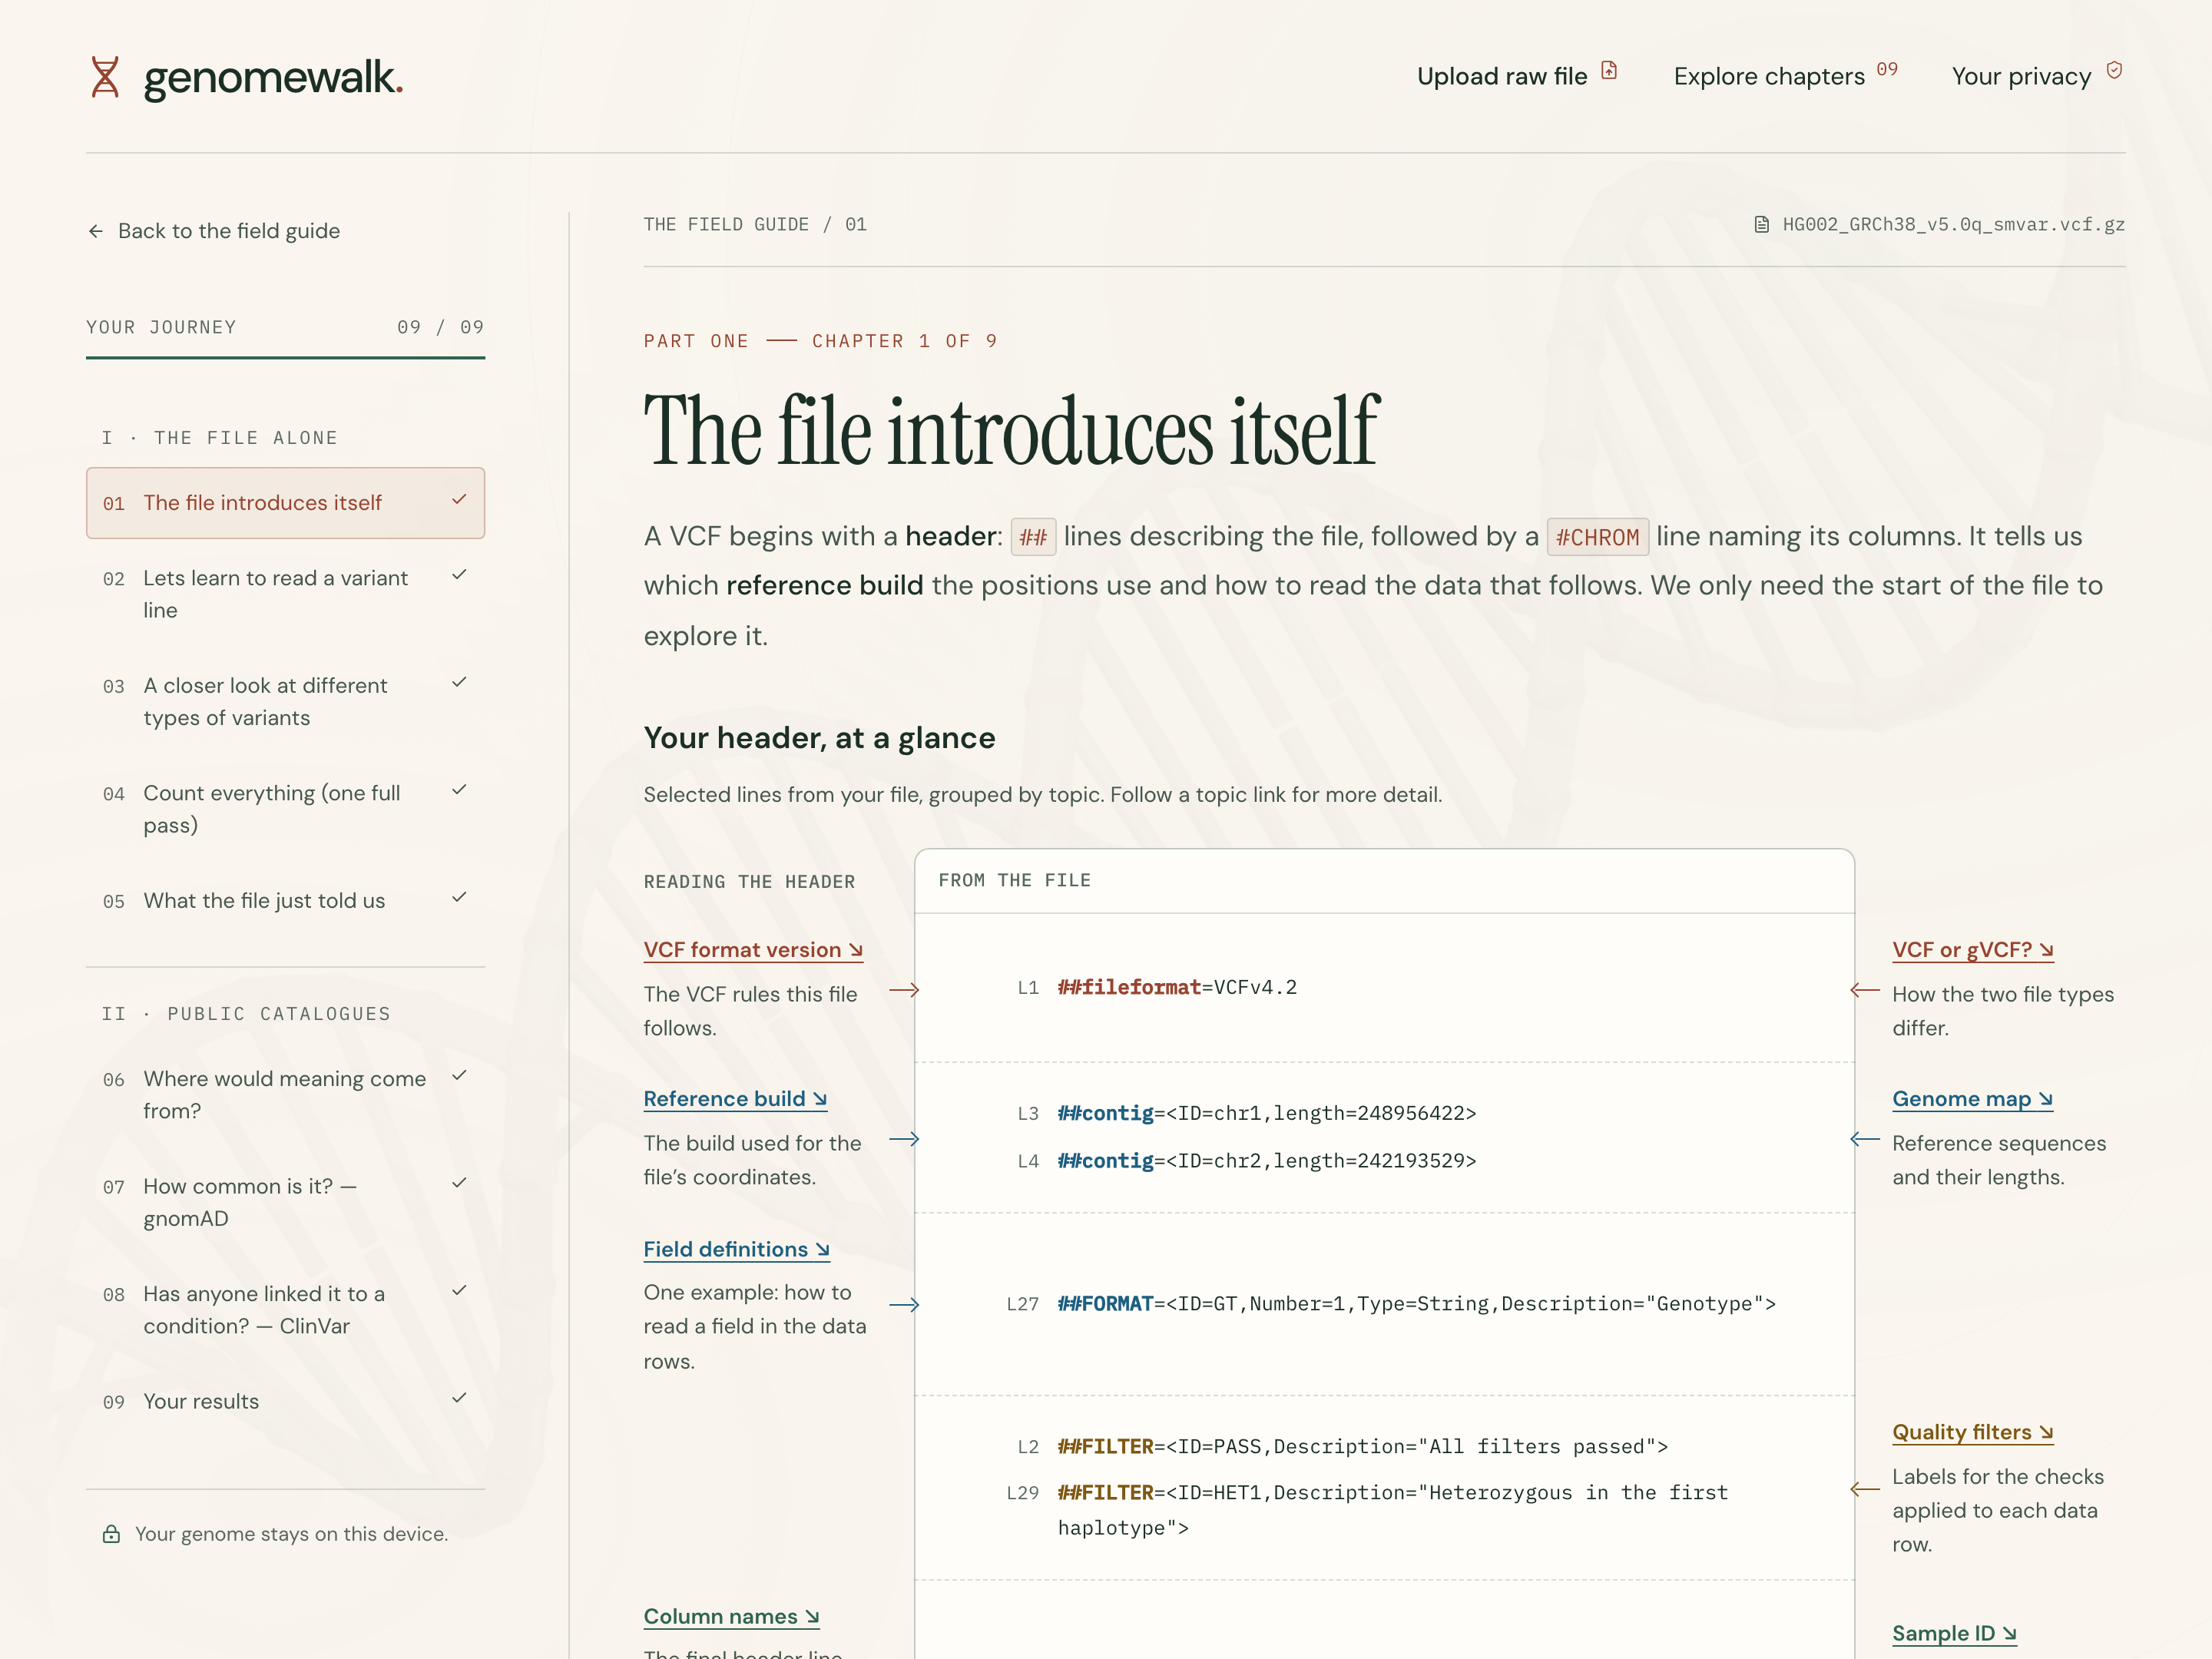
\includegraphics[width=\linewidth]{figures/chapters/chapter-01-desktop.png}
\Description{Full desktop view of Chapter 1 with the chapter navigation, HG002 filename, and an annotated header display linking selected VCF lines to explanations of format, reference build and field definitions.}
\caption{Chapter 1 introduces the selected HG002 file through labelled excerpts from its header.}
\label{fig:chapter-1}
\end{wrapfigure}
The reader begins with the file header (Fig.~\ref{fig:chapter-1}). Selected lines are arranged beside explanations of the VCF version, reference build, field definitions, filters and column names. Topic links lead to more detail about the corresponding lines. For HG002, this includes the GRCh38 reference and the sample column. The chapter establishes how to read the file's own description before interpreting its variant records, including why a chromosome and position need a reference build.
\finishchapterwrap
\end{minipage}\par


\par\noindent\begin{minipage}{\textwidth}
\subsection{Chapter 2: Let's learn to read a variant line}
\setlength{\intextsep}{4pt}
\setlength{\columnsep}{.04\textwidth}
\begin{wrapfigure}{r}{.50\textwidth}
\centering
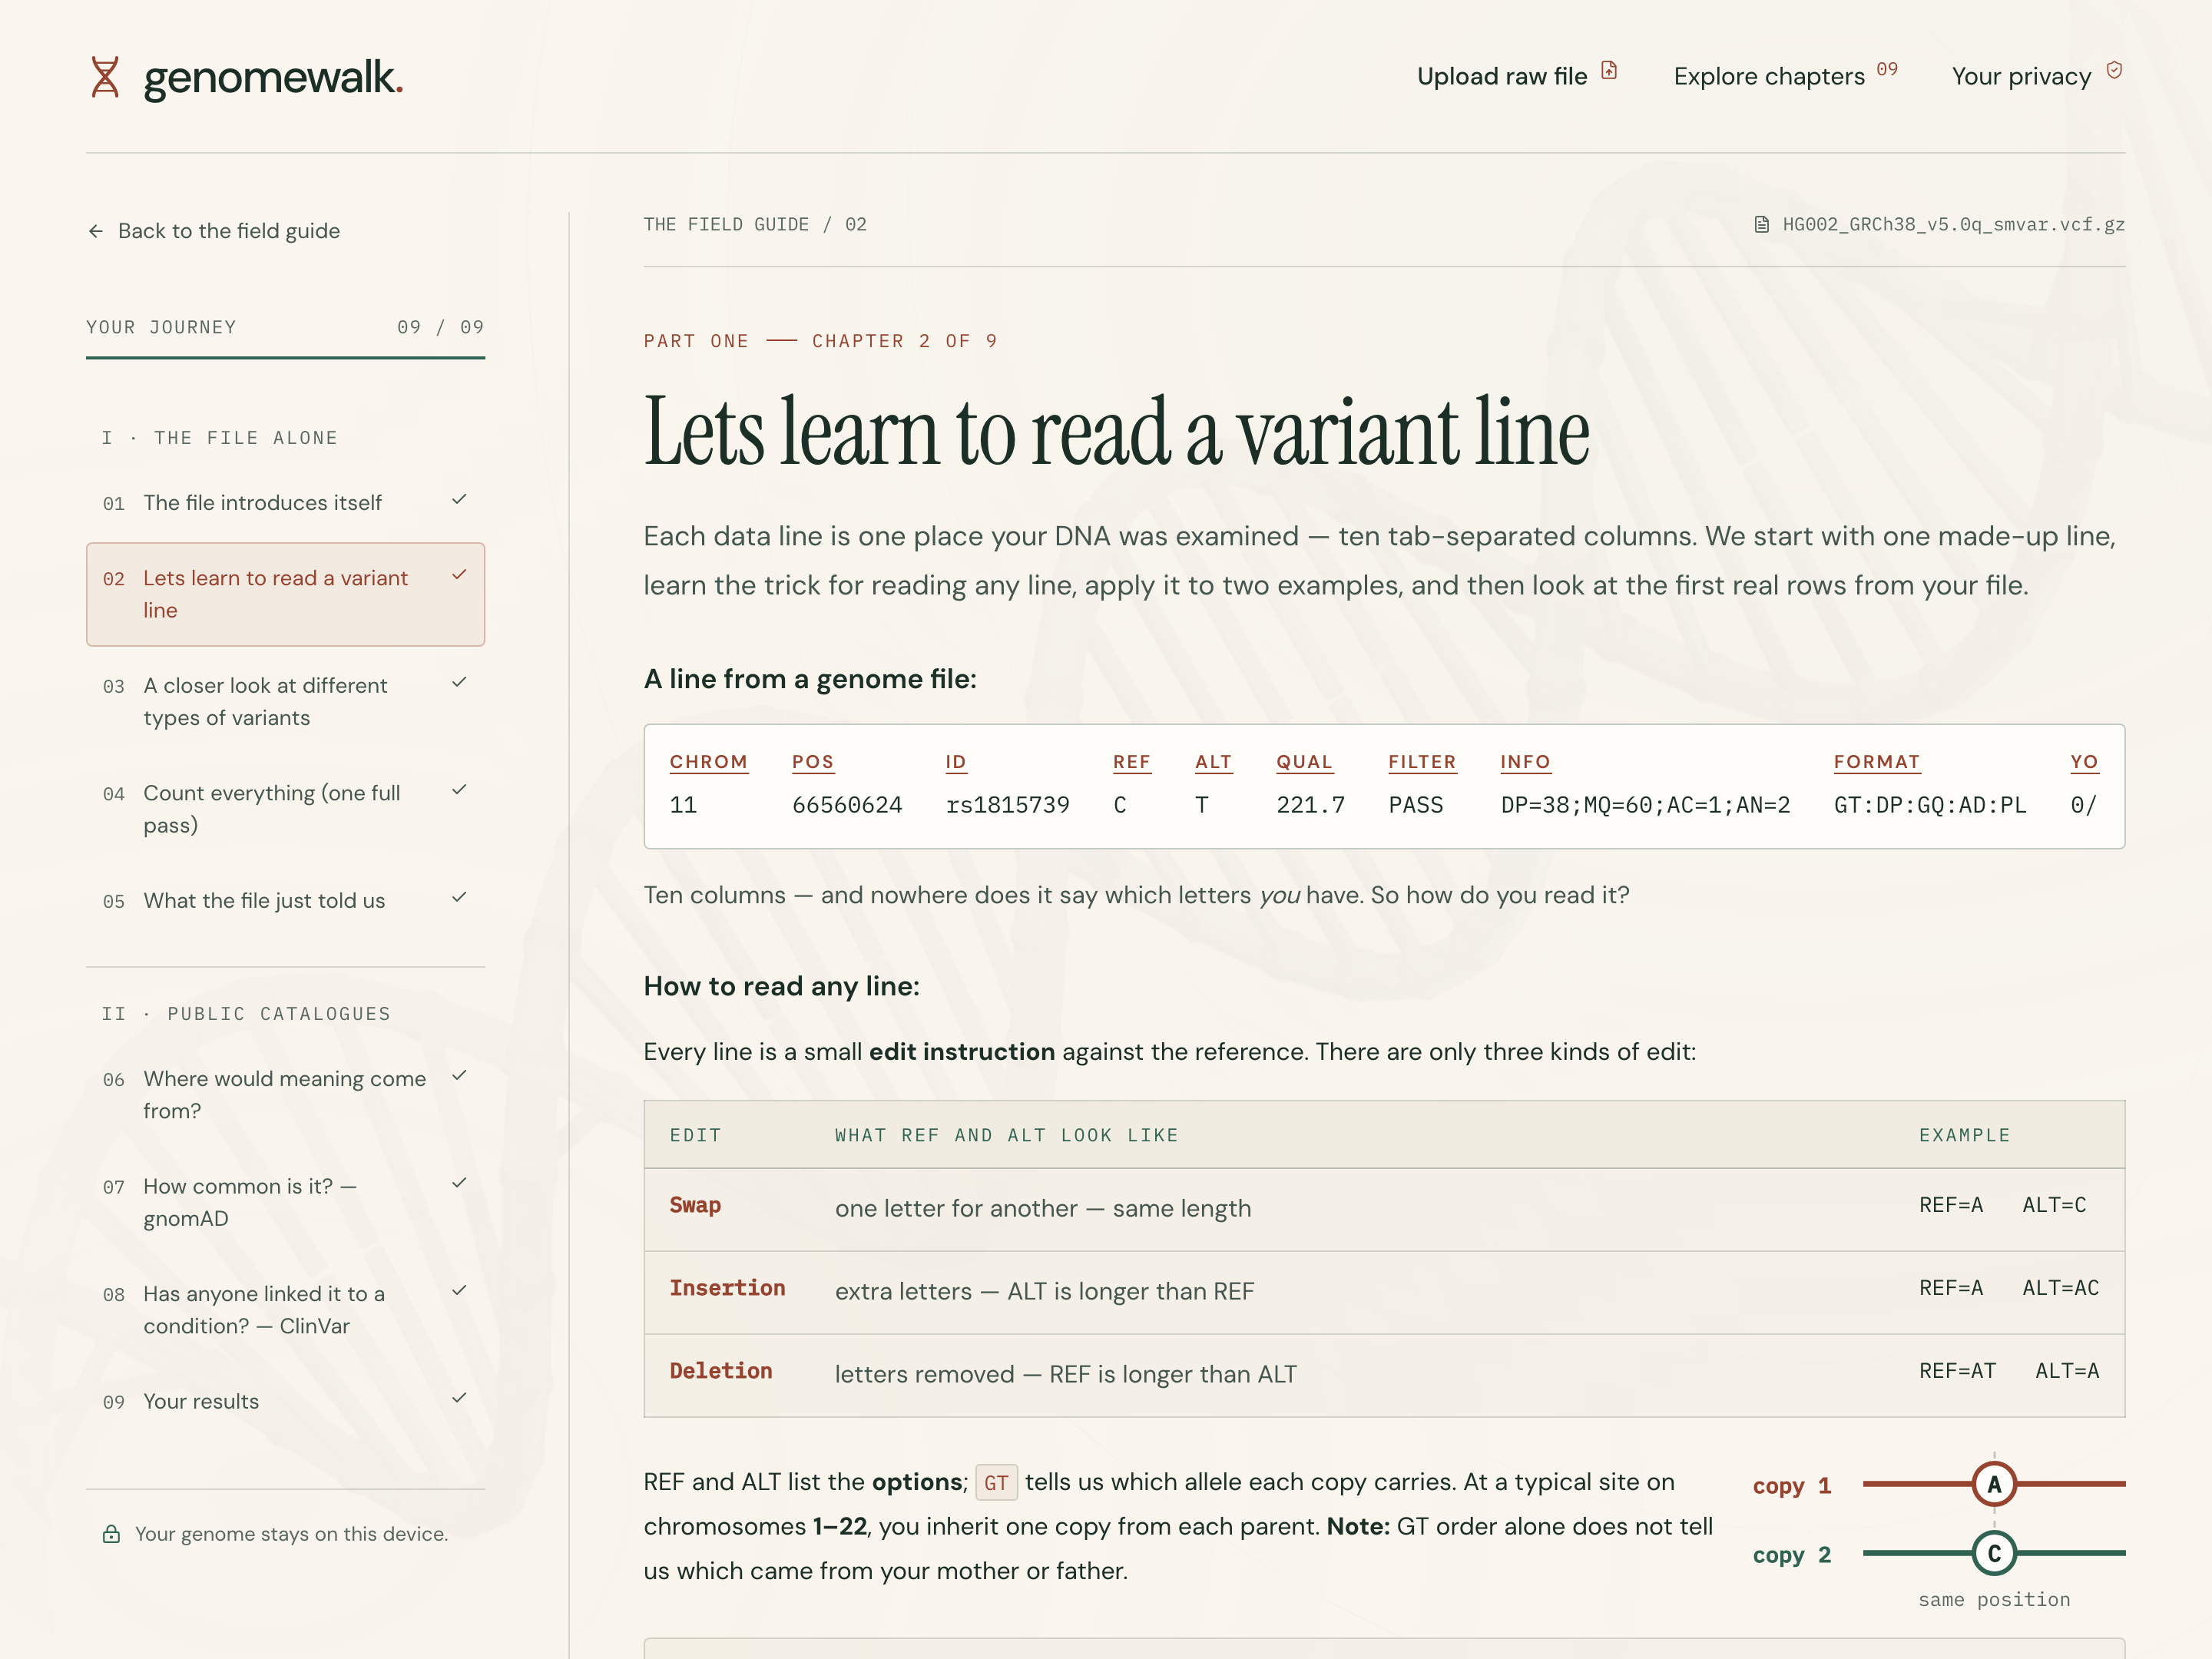
\includegraphics[width=\linewidth]{figures/chapters/chapter-02-desktop.png}
\Description{Full desktop view of Chapter 2 showing a constructed variant row, a comparison of substitutions, insertions and deletions, and a two-copy allele illustration. The selected file is HG002, but this introductory row is a teaching example.}
\caption{Chapter 2 begins with a constructed example; selected-file rows follow later in the chapter.}
\label{fig:chapter-2}
\end{wrapfigure}
This chapter starts with a constructed teaching row and then applies the same reading procedure to rows from the selected file (Fig.~\ref{fig:chapter-2}). Reference and alternate alleles describe sequence options; the genotype identifies the called alleles. Small diagrams explain substitutions, insertions, deletions and chromosome copies. Later, an actual HG002 row at chromosome 1 position 89177 illustrates how genotype \texttt{1|1} selects the alternate G allele for both copies. The explanation also distinguishes phasing from identifying a parent.
\finishchapterwrap
\end{minipage}\par


\par\noindent\begin{minipage}{\textwidth}
\subsection{Chapter 3: A closer look at different types of variants}
\setlength{\intextsep}{4pt}
\setlength{\columnsep}{.04\textwidth}
\begin{wrapfigure}{r}{.50\textwidth}
\centering
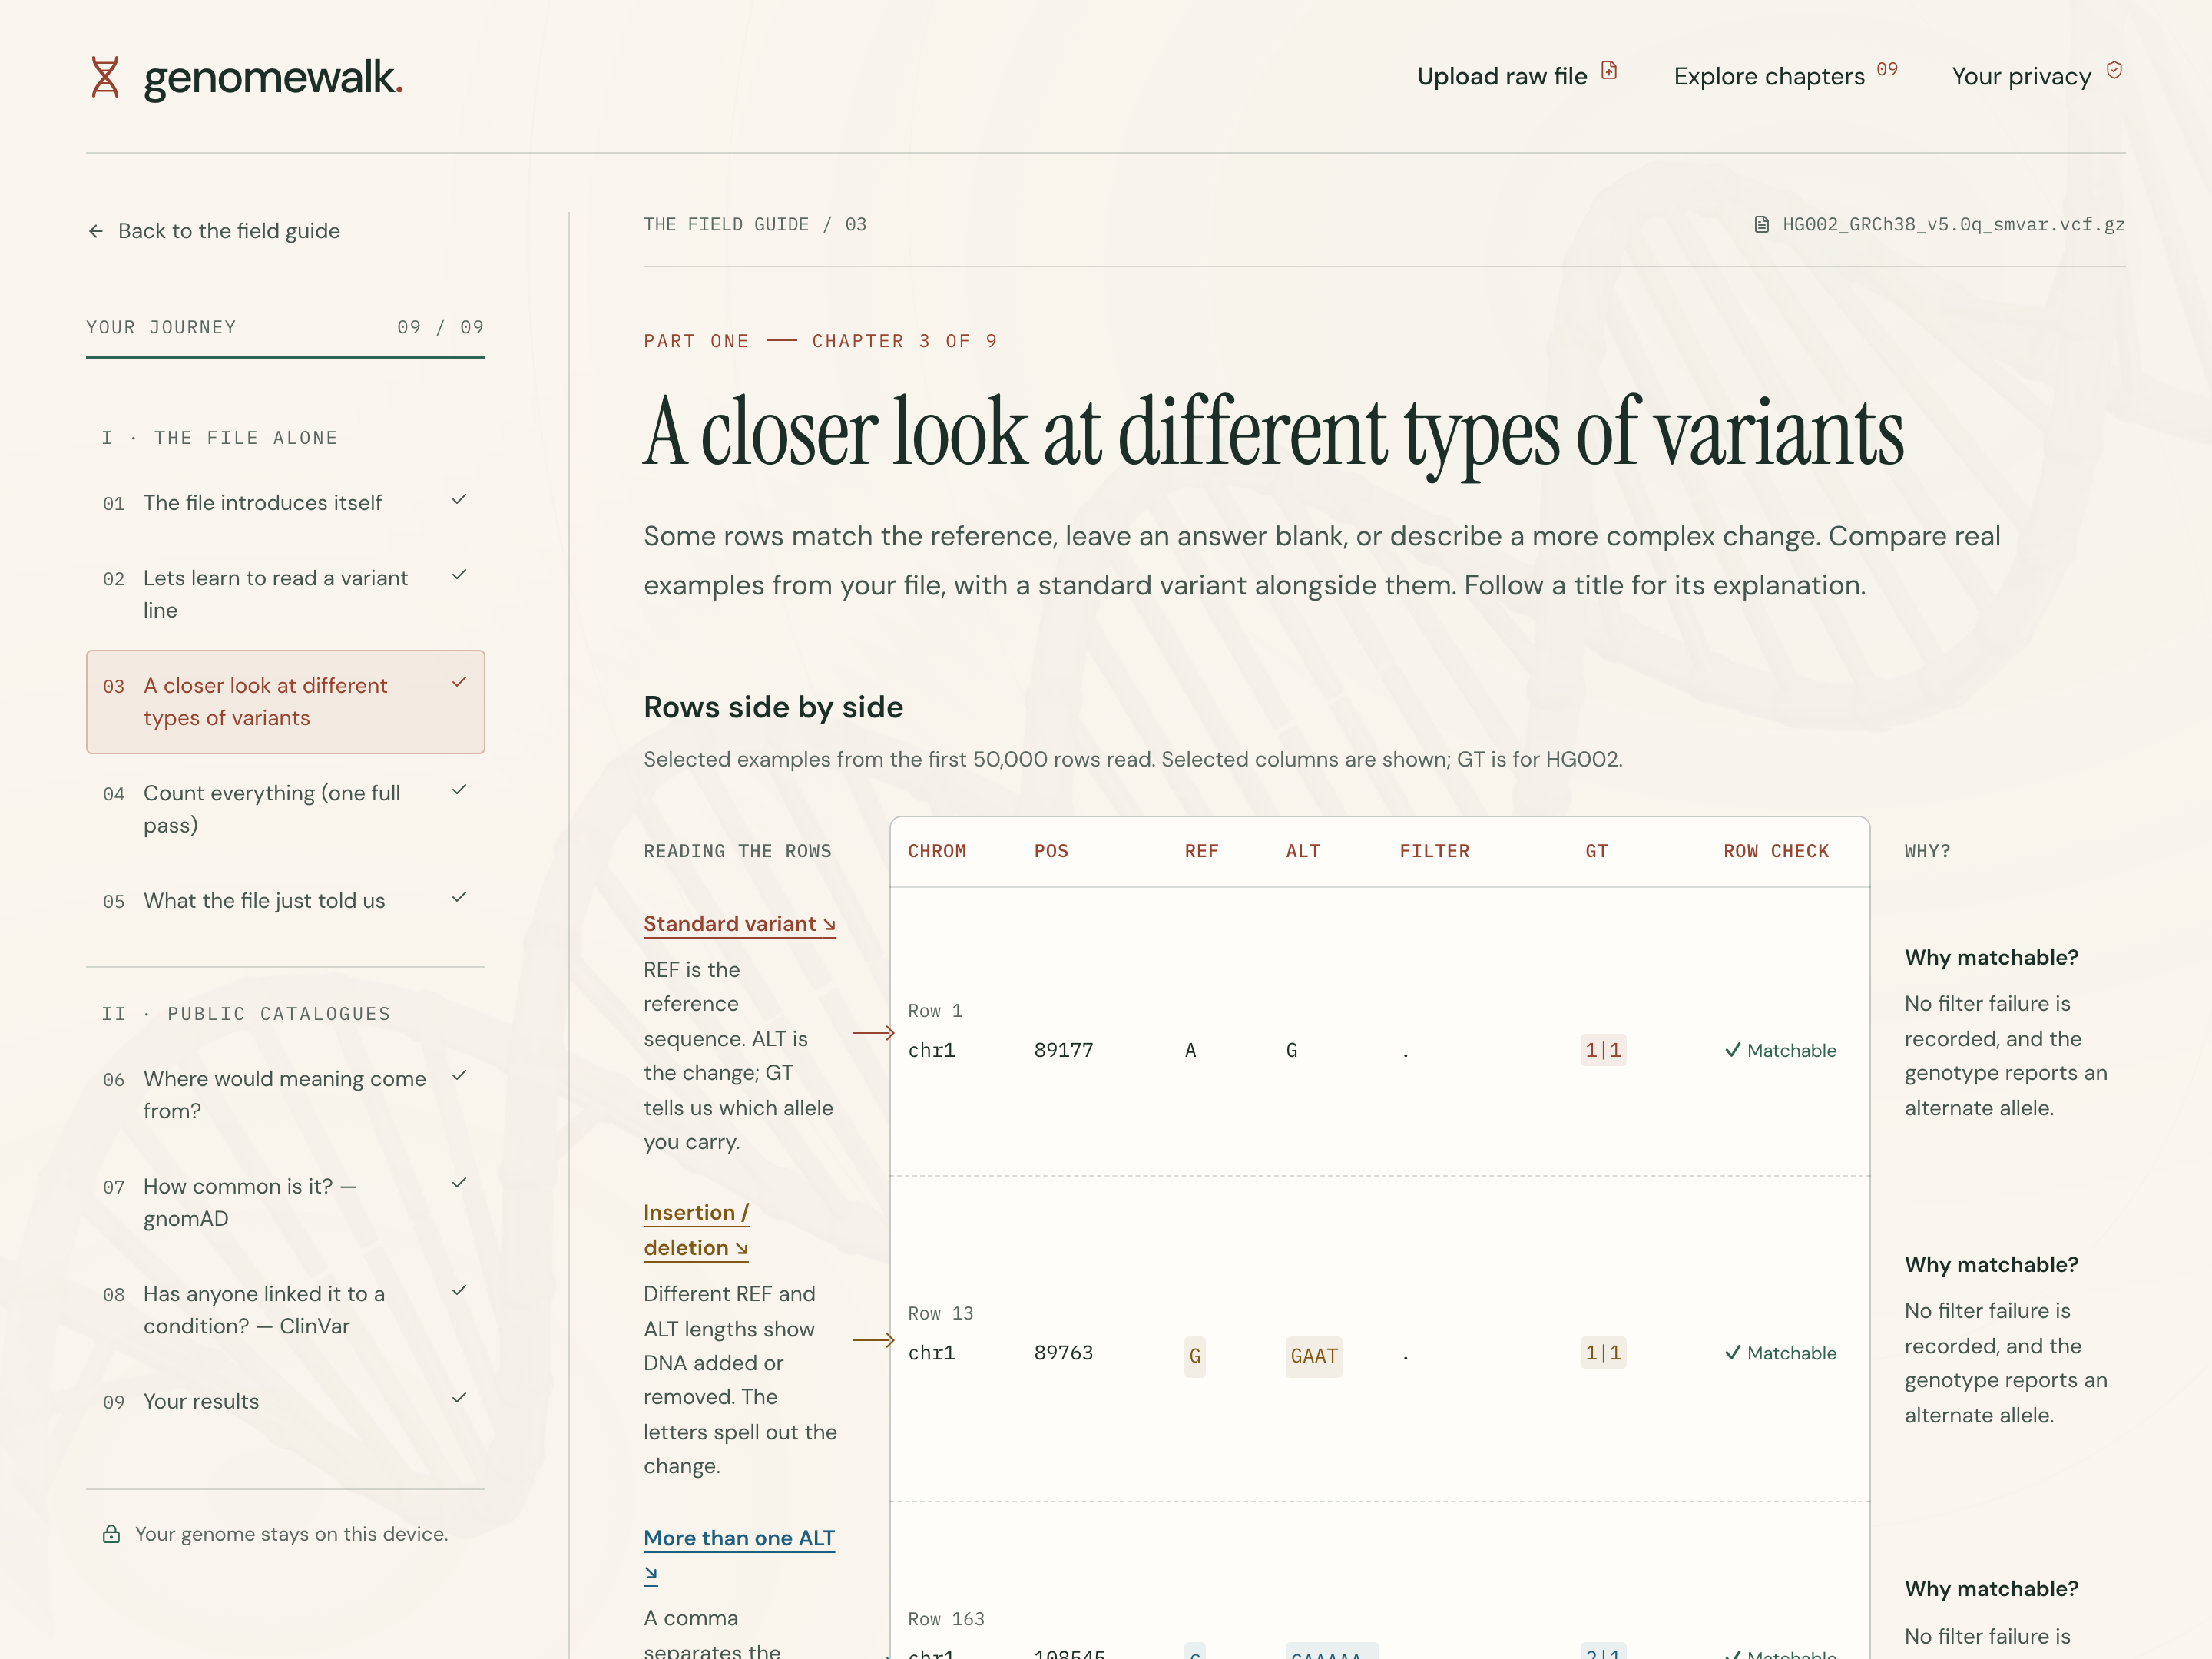
\includegraphics[width=\linewidth]{figures/chapters/chapter-03-desktop.png}
\Description{Full desktop view of Chapter 3 comparing selected HG002 records, including a single-base substitution, an insertion and a multiallelic site, with genotype and matching explanations.}
\caption{Chapter 3 compares variant representations found in the selected HG002 file.}
\label{fig:chapter-3}
\end{wrapfigure}
The reader next compares examples selected from the first 50,000 rows read from the file (Fig.~\ref{fig:chapter-3}). The HG002 view includes a single-base substitution, an insertion and a site with multiple alternate alleles. Each example retains its genotype and explains the relationship between the allele strings and the call. Notes on matching indicate which representations the application can use. This moves the reader beyond a single simple row while keeping the examples grounded in the selected file.
\finishchapterwrap
\end{minipage}\par


\par\noindent\begin{minipage}{\textwidth}
\subsection{Chapter 4: Count everything (one full pass)}
\setlength{\intextsep}{4pt}
\setlength{\columnsep}{.04\textwidth}
\begin{wrapfigure}{r}{.50\textwidth}
\centering
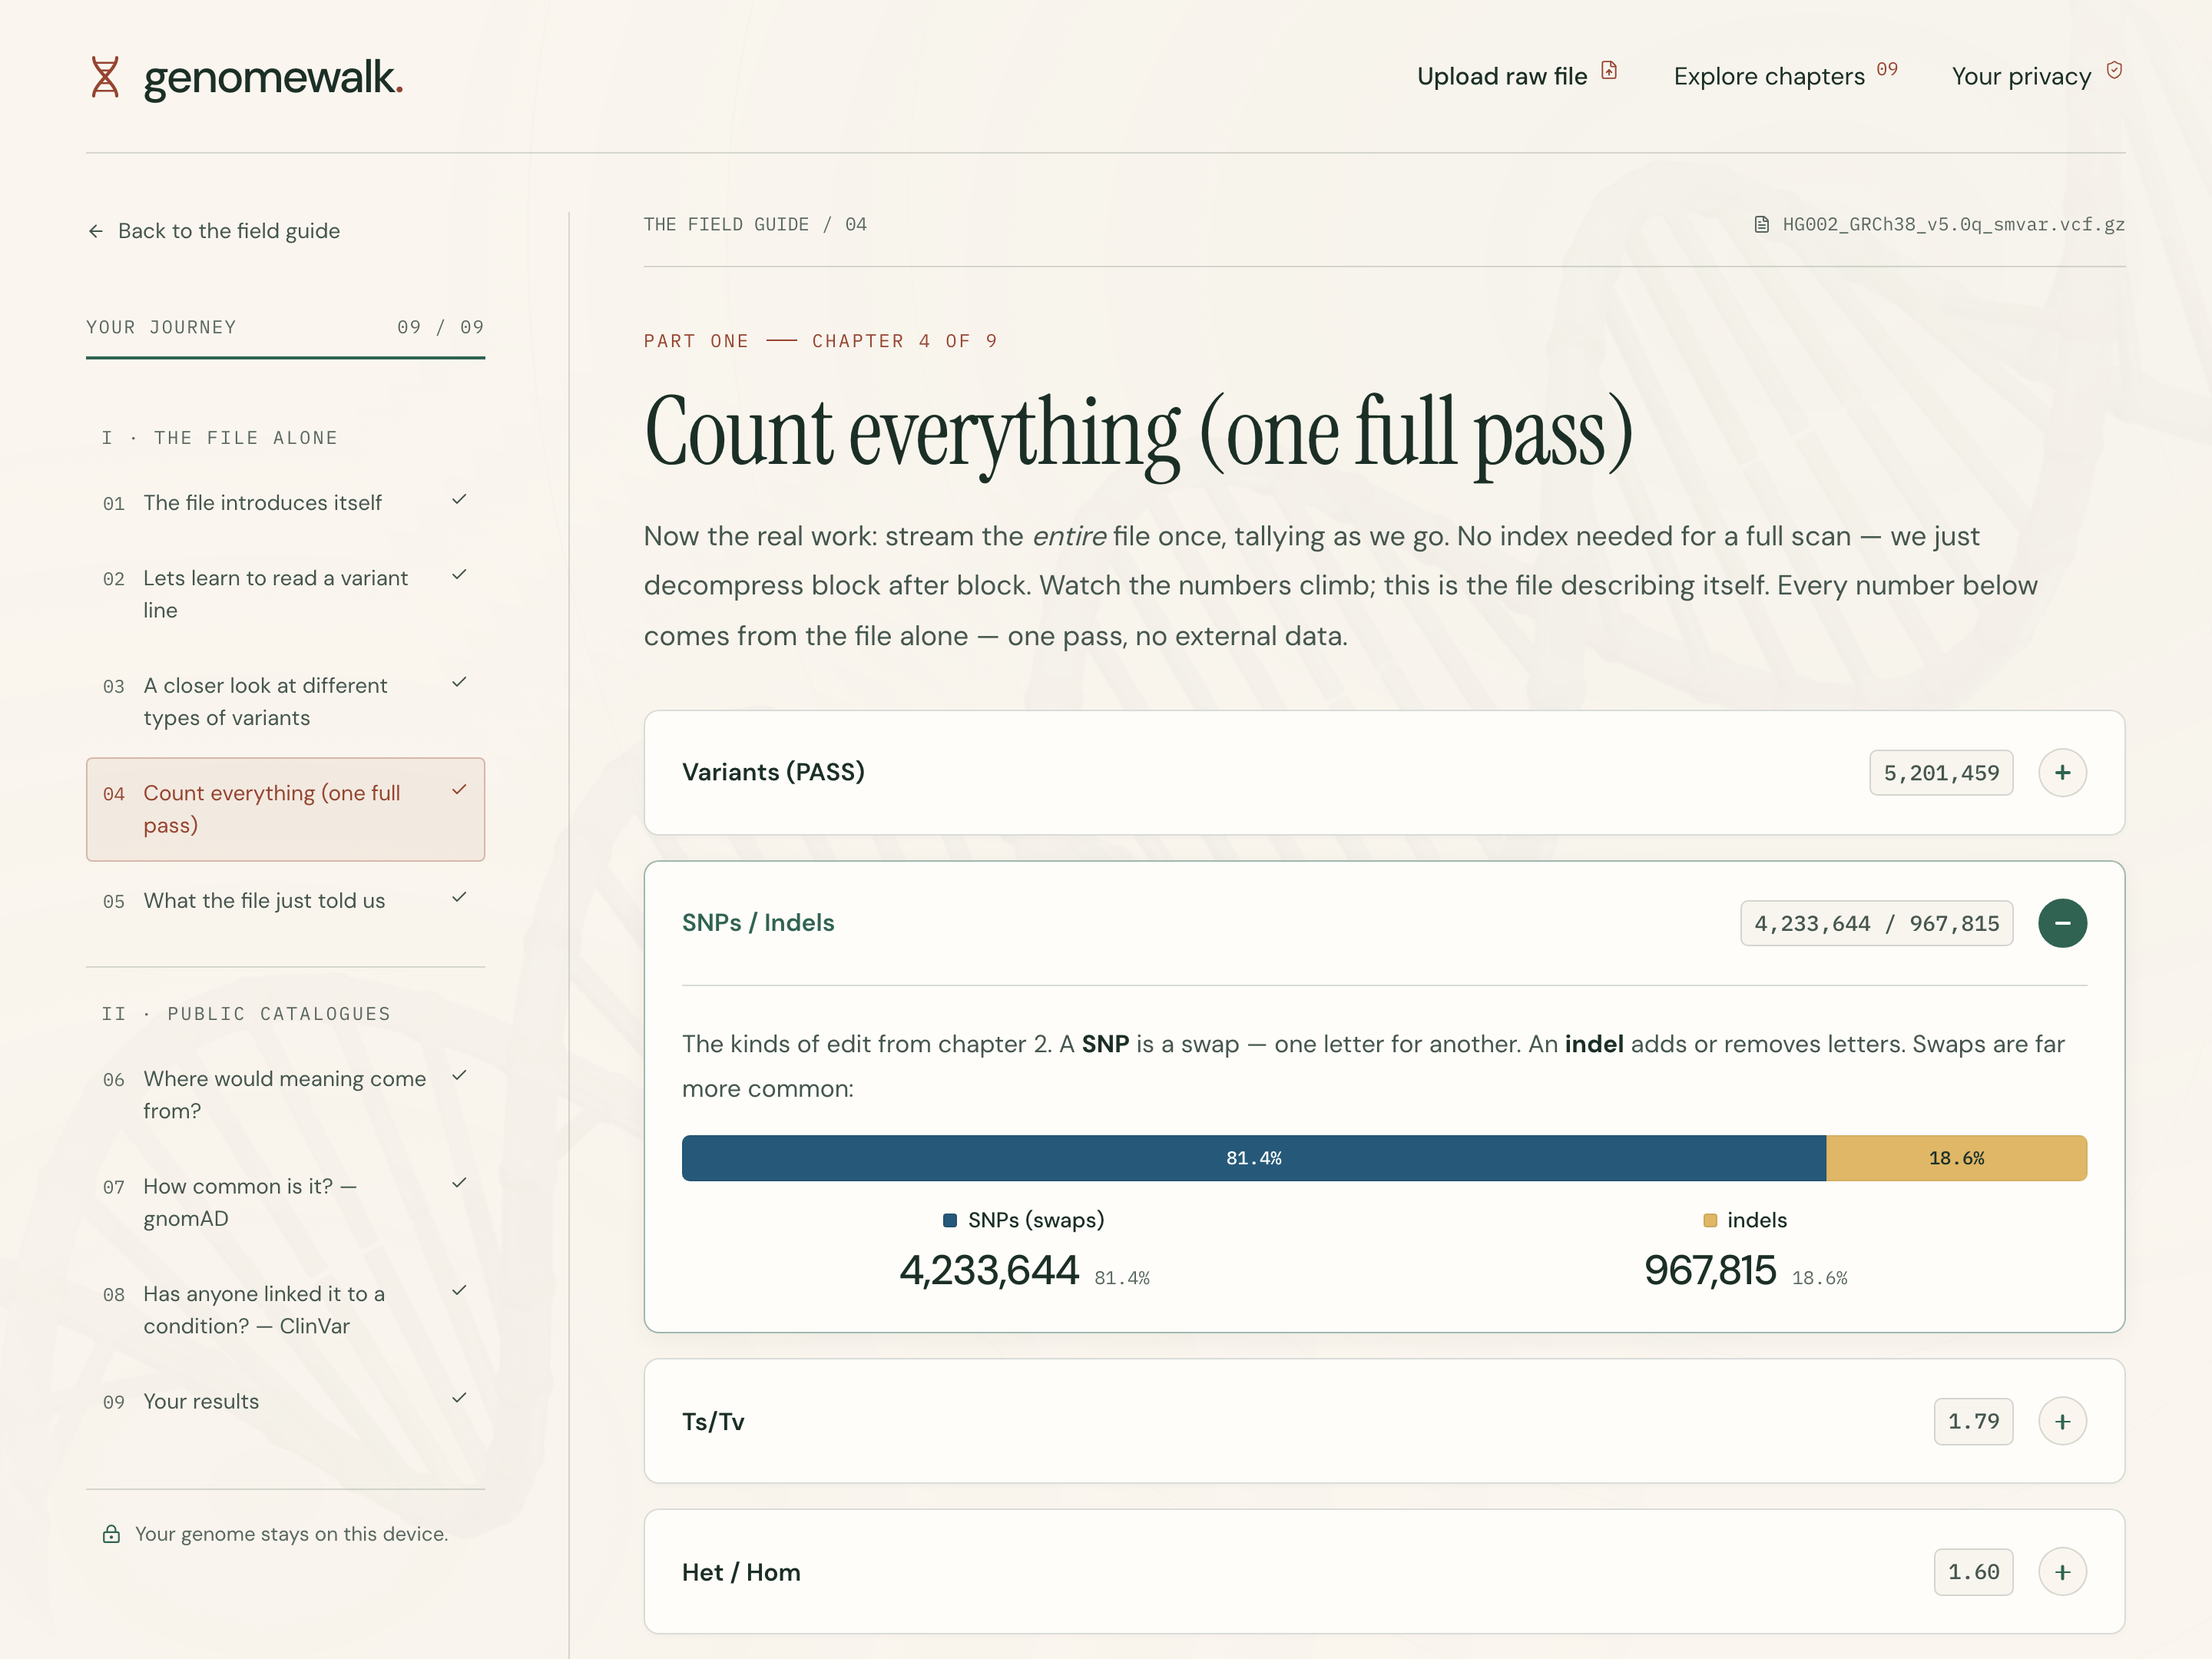
\includegraphics[width=\linewidth]{figures/chapters/chapter-04-desktop.png}
\Description{Full desktop view of Chapter 4 after the HG002 scan, showing file statistics and the expanded SNP/indel breakdown with 4,233,644 SNPs and 967,815 indels.}
\caption{Chapter 4 summarizes a complete HG002 scan, with the SNP/indel explanation expanded.}
\label{fig:chapter-4}
\end{wrapfigure}
This chapter scans the complete file and summarizes what it contains (Fig.~\ref{fig:chapter-4}). Readers can inspect variant counts, the balance of substitutions and indels, and other available file statistics. Expandable explanations connect each measure to its meaning; the screenshot opens the SNP/indel breakdown. The HG002 scan reports 5,201,459 counted variant rows, including 4,233,644 SNPs and 967,815 indels. These are descriptions of the input records, not counts of health findings. Information absent from the file remains visibly unavailable.
\finishchapterwrap
\end{minipage}\par


\par\noindent\begin{minipage}{\textwidth}
\subsection{Chapter 5: What the file just told us}
\setlength{\intextsep}{4pt}
\setlength{\columnsep}{.04\textwidth}
\begin{wrapfigure}{r}{.50\textwidth}
\centering
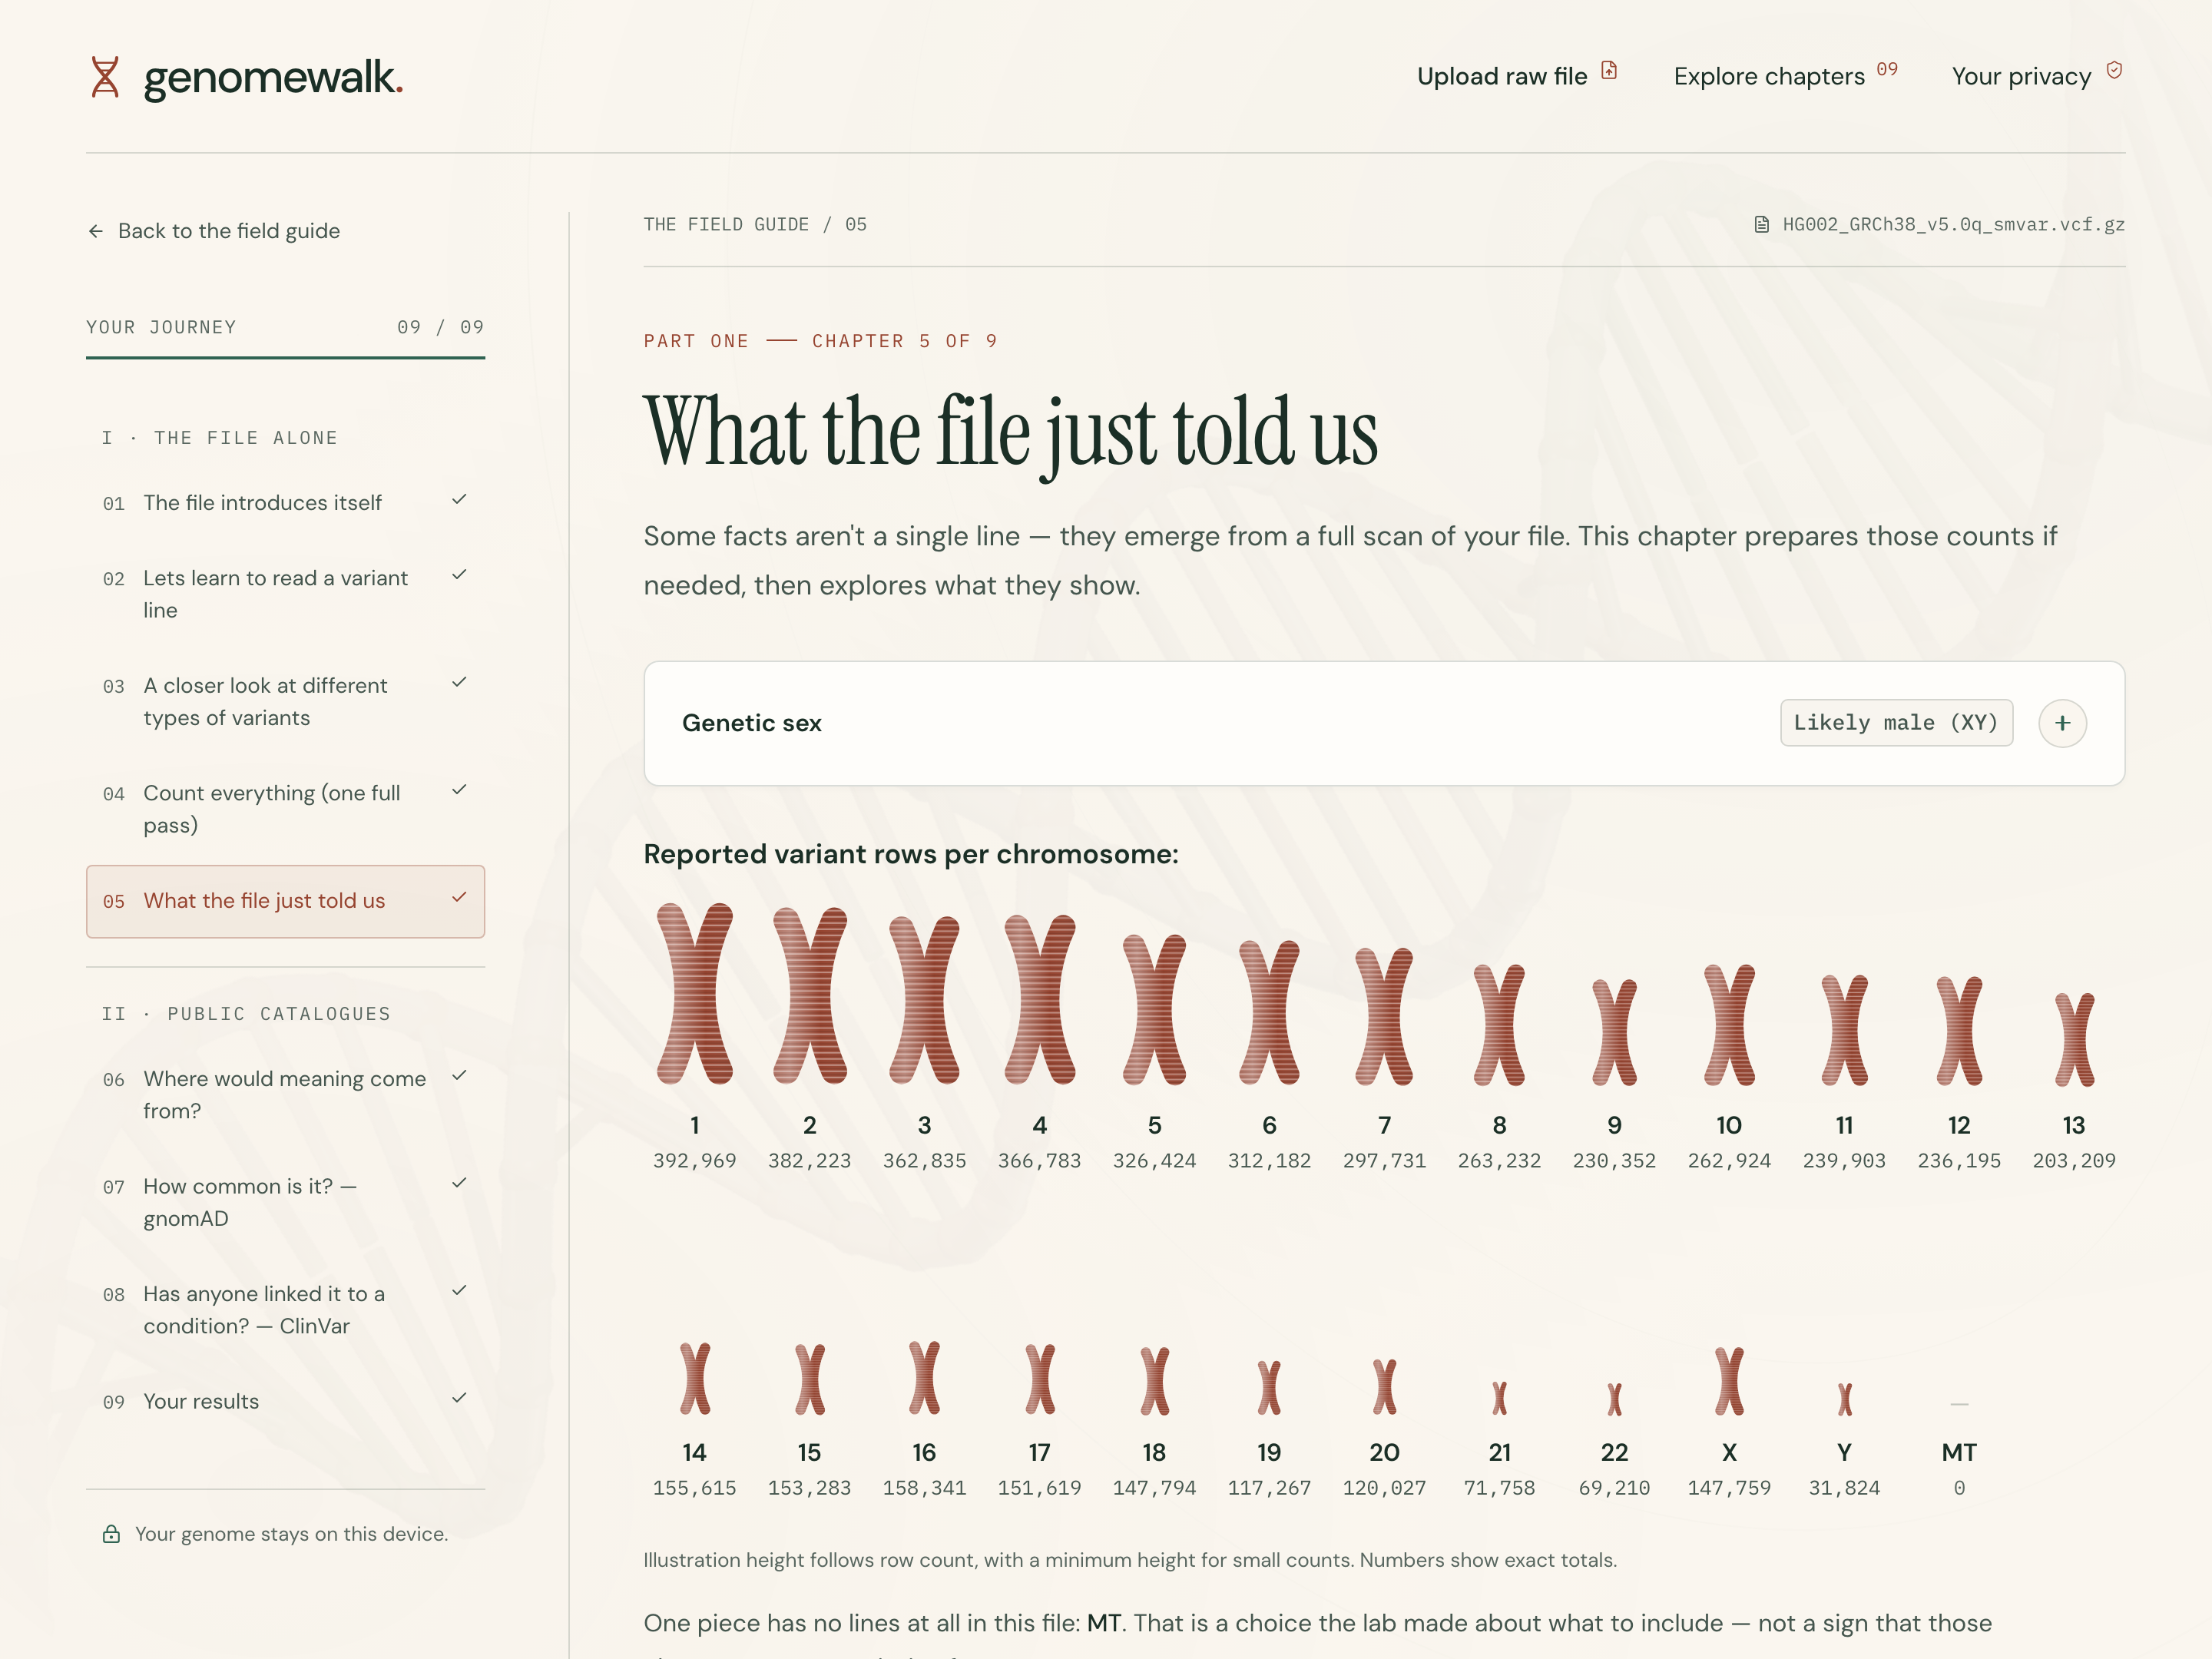
\includegraphics[width=\linewidth]{figures/chapters/chapter-05-desktop.png}
\Description{Full desktop view of Chapter 5 with a chromosome overview showing the distribution of variant records reported in the HG002 file, including a zero mitochondrial variant count.}
\caption{Chapter 5 summarizes file observations; chromosome counts describe reported records, not chromosome size or completeness.}
\label{fig:chapter-5}
\end{wrapfigure}
The final chapter of the first part brings the file observations together (Fig.~\ref{fig:chapter-5}). A chromosome overview shows how the counted variant rows are distributed across the genome. Readers can compare counts while considering what the file contains and what it does not report. In the HG002 view, the mitochondrial variant count in this summary is zero; this does not mean the sample lacks mitochondrial DNA. The chapter closes the file-reading sequence before introducing public evidence.
\finishchapterwrap
\end{minipage}\par


\par\noindent\begin{minipage}{\textwidth}
\subsection{Chapter 6: Where would meaning come from?}
\setlength{\intextsep}{4pt}
\setlength{\columnsep}{.04\textwidth}
\begin{wrapfigure}{r}{.50\textwidth}
\centering
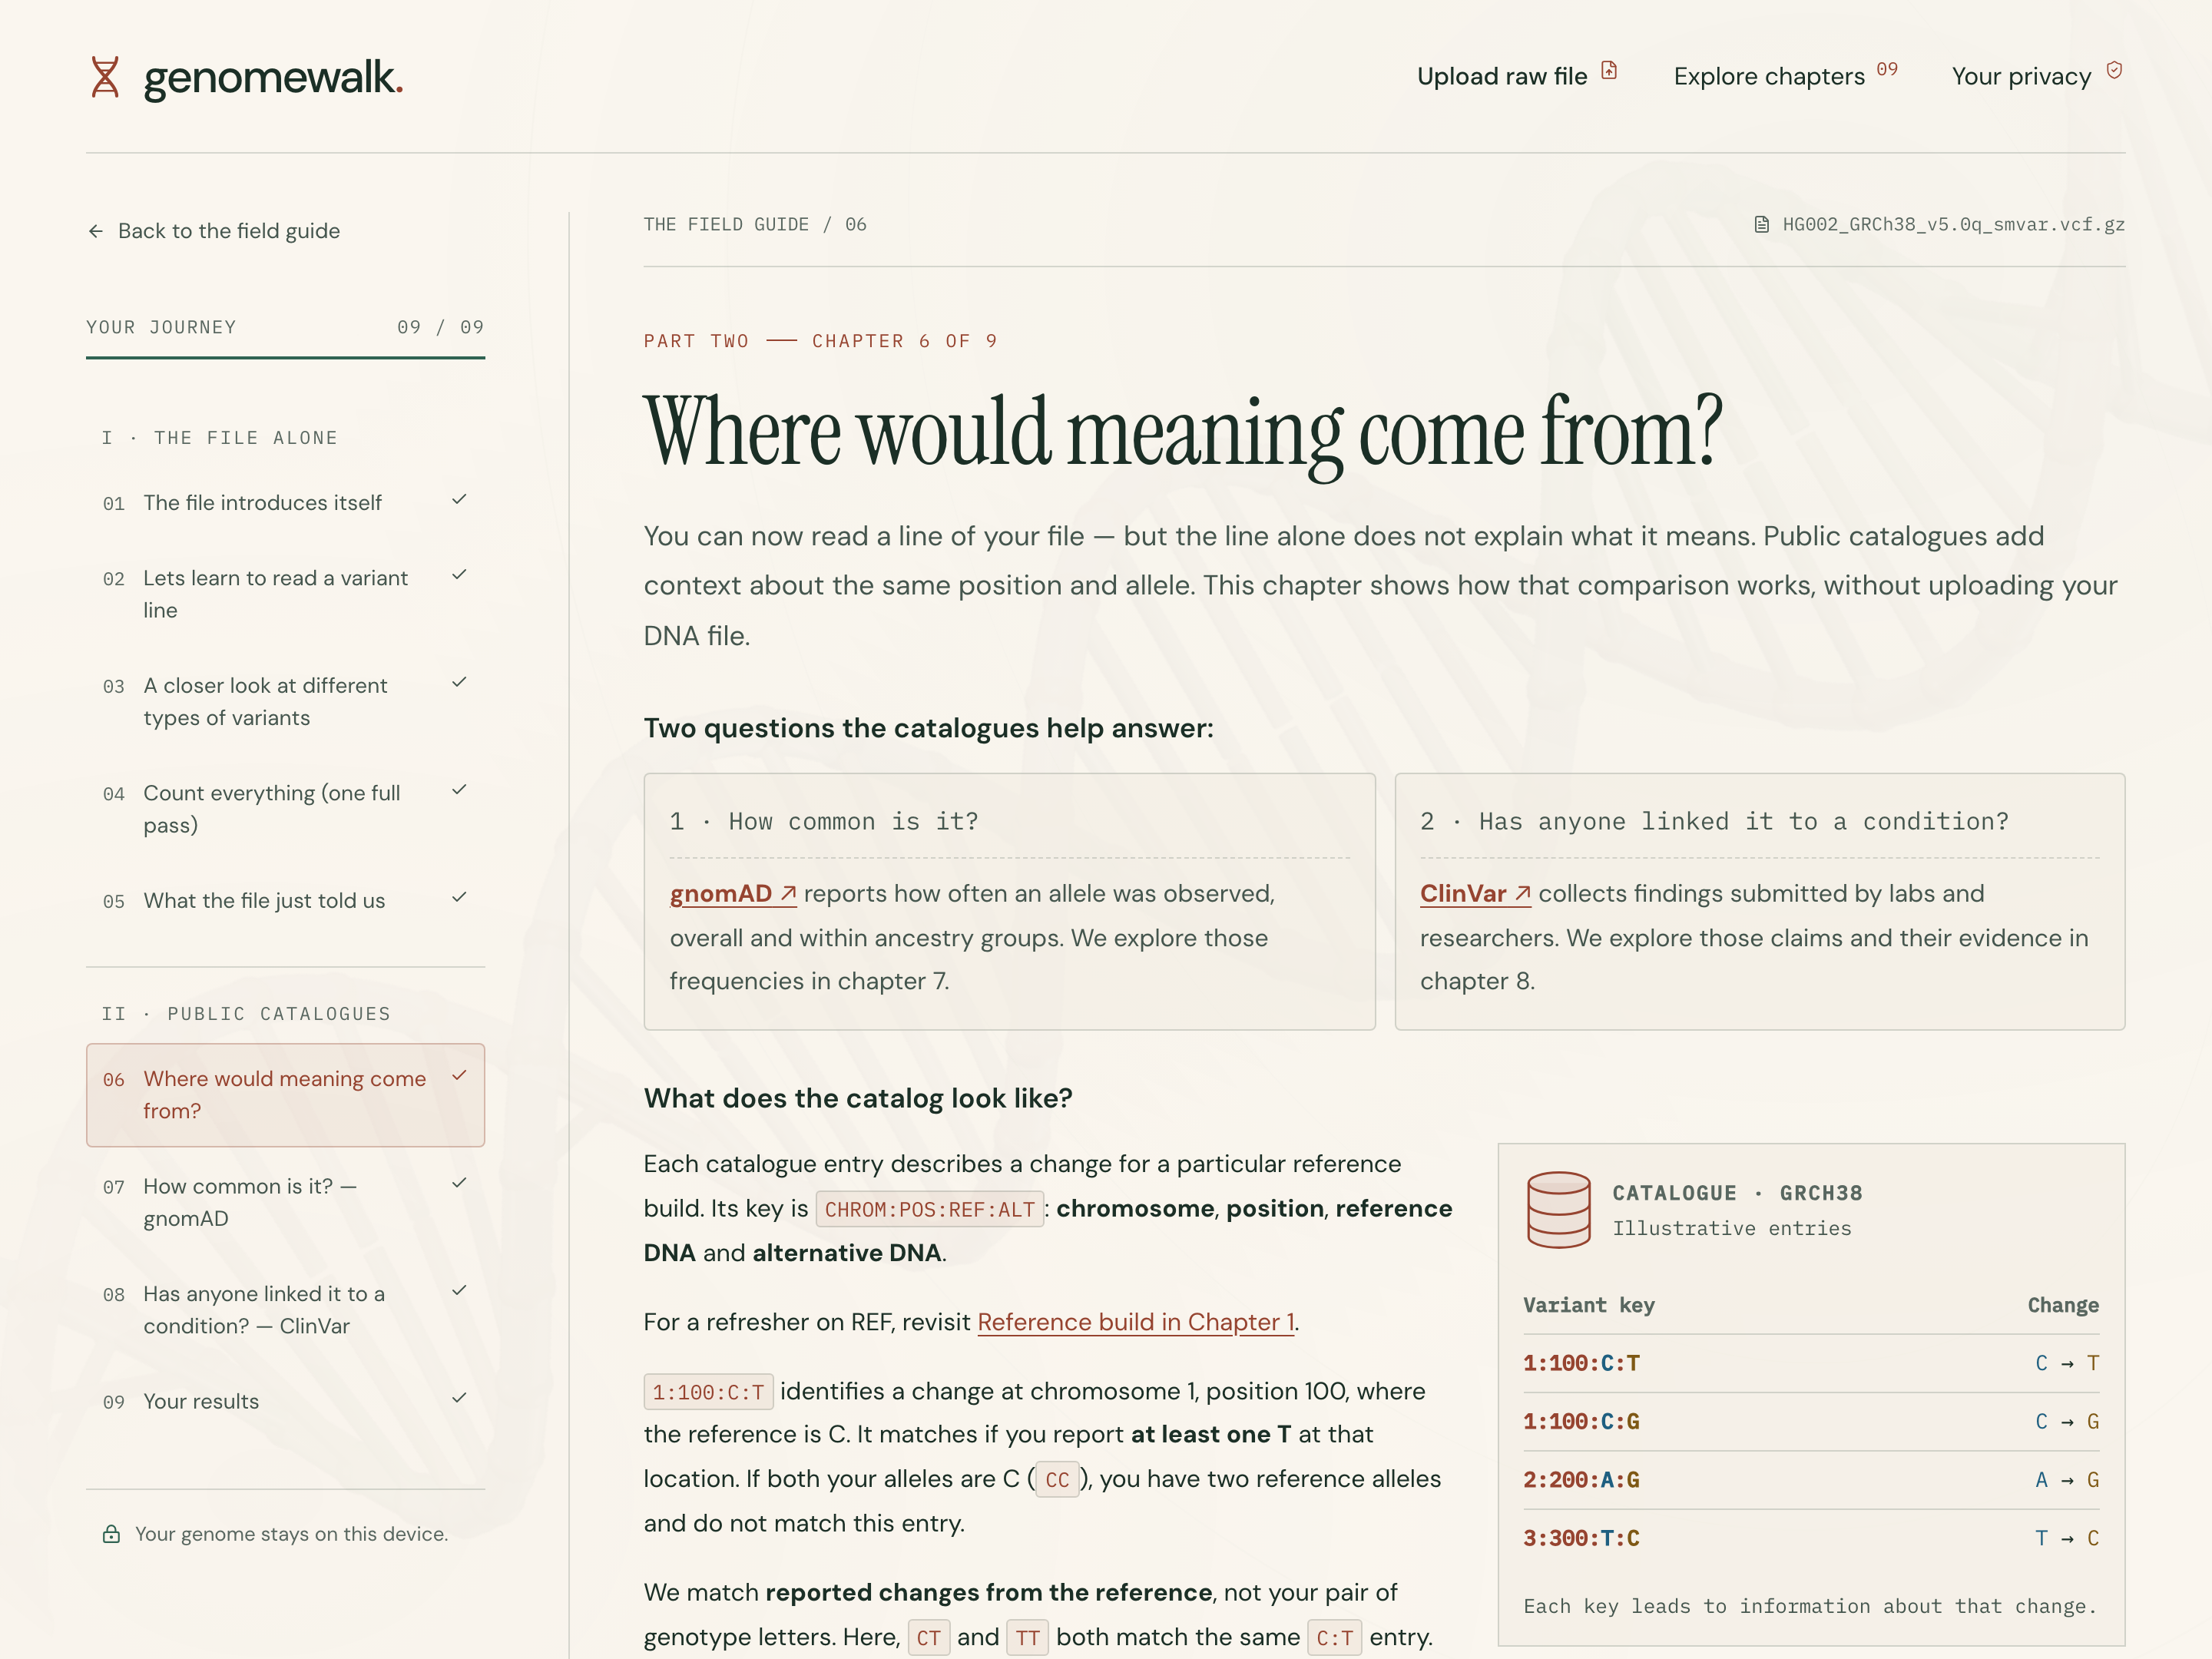
\includegraphics[width=\linewidth]{figures/chapters/chapter-06-desktop.png}
\Description{Full desktop view of Chapter 6 introducing population frequency and public classifications, followed by illustrative catalogue entries and their chromosome-position-reference-alternate keys.}
\caption{Chapter 6 introduces public evidence and catalogue matching using illustrative entries.}
\label{fig:chapter-6}
\end{wrapfigure}
The second part begins by separating two questions: how common an allele is, and what claims have been made about it (Fig.~\ref{fig:chapter-6}). The chapter introduces gnomAD and ClinVar as sources for those questions. An illustrative catalogue explains how chromosome, position, reference and alternate allele identify a public record within a reference build. Genotype examples show why different calls can refer to the same catalogue allele. These examples introduce the matching process; they are not presented as HG002 findings.
\finishchapterwrap
\end{minipage}\par


\par\noindent\begin{minipage}{\textwidth}
\subsection{Chapter 7: How common is it?---gnomAD}
\setlength{\intextsep}{4pt}
\setlength{\columnsep}{.04\textwidth}
\begin{wrapfigure}{r}{.50\textwidth}
\centering
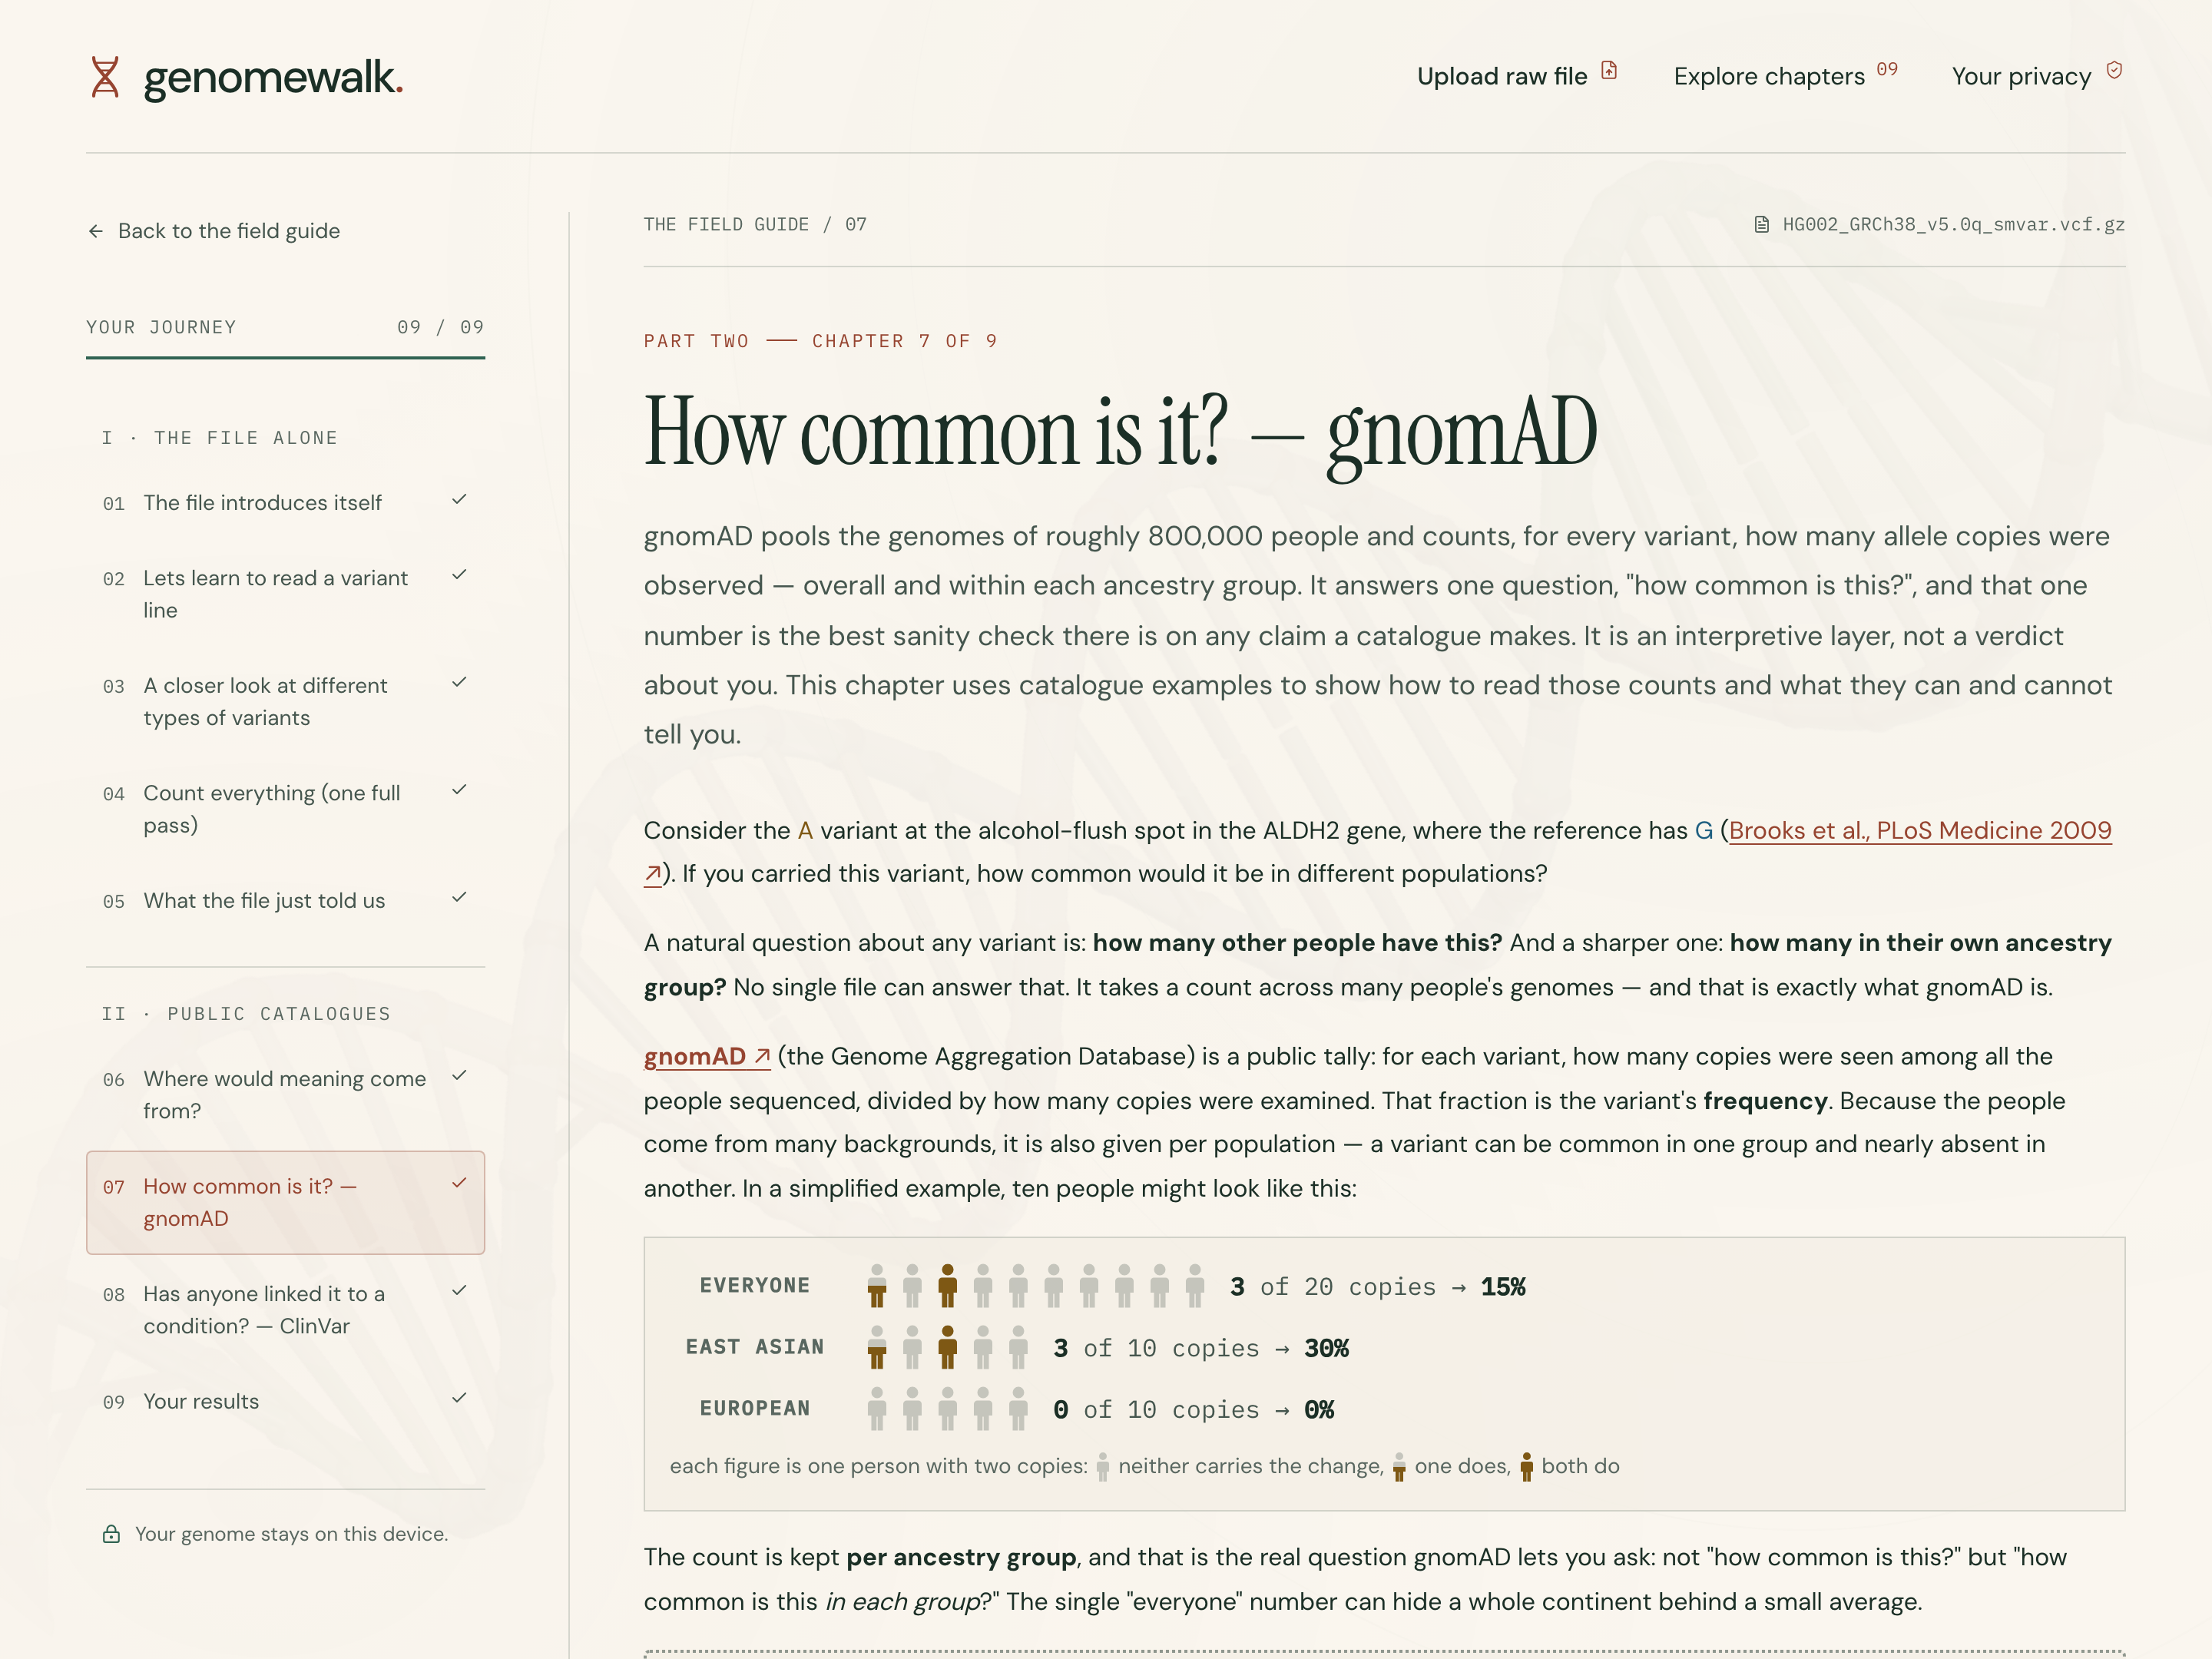
\includegraphics[width=\linewidth]{figures/chapters/chapter-07-desktop.png}
\Description{Full desktop view of Chapter 7 showing a simplified allele-count illustration with combined and population-group frequencies. The counts are teaching examples, not frequencies calculated from HG002.}
\caption{Chapter 7 uses illustrative allele counts to explain population frequency and its denominator.}
\label{fig:chapter-7}
\end{wrapfigure}
This chapter explains population frequency by counting allele copies (Fig.~\ref{fig:chapter-7}). A simplified illustration compares a combined group with smaller population groups, before relating the idea to public catalogue examples. Readers see why the denominator matters and why frequencies can differ between groups. The figures illustrate the concept rather than measuring HG002. The chapter treats frequency as context about observed allele copies, distinct from a person's probability of developing a condition.
\finishchapterwrap
\end{minipage}\par


\par\noindent\begin{minipage}{\textwidth}
\subsection{Chapter 8: Has anyone linked it to a condition?---ClinVar}
\setlength{\intextsep}{4pt}
\setlength{\columnsep}{.04\textwidth}
\begin{wrapfigure}{r}{.50\textwidth}
\centering
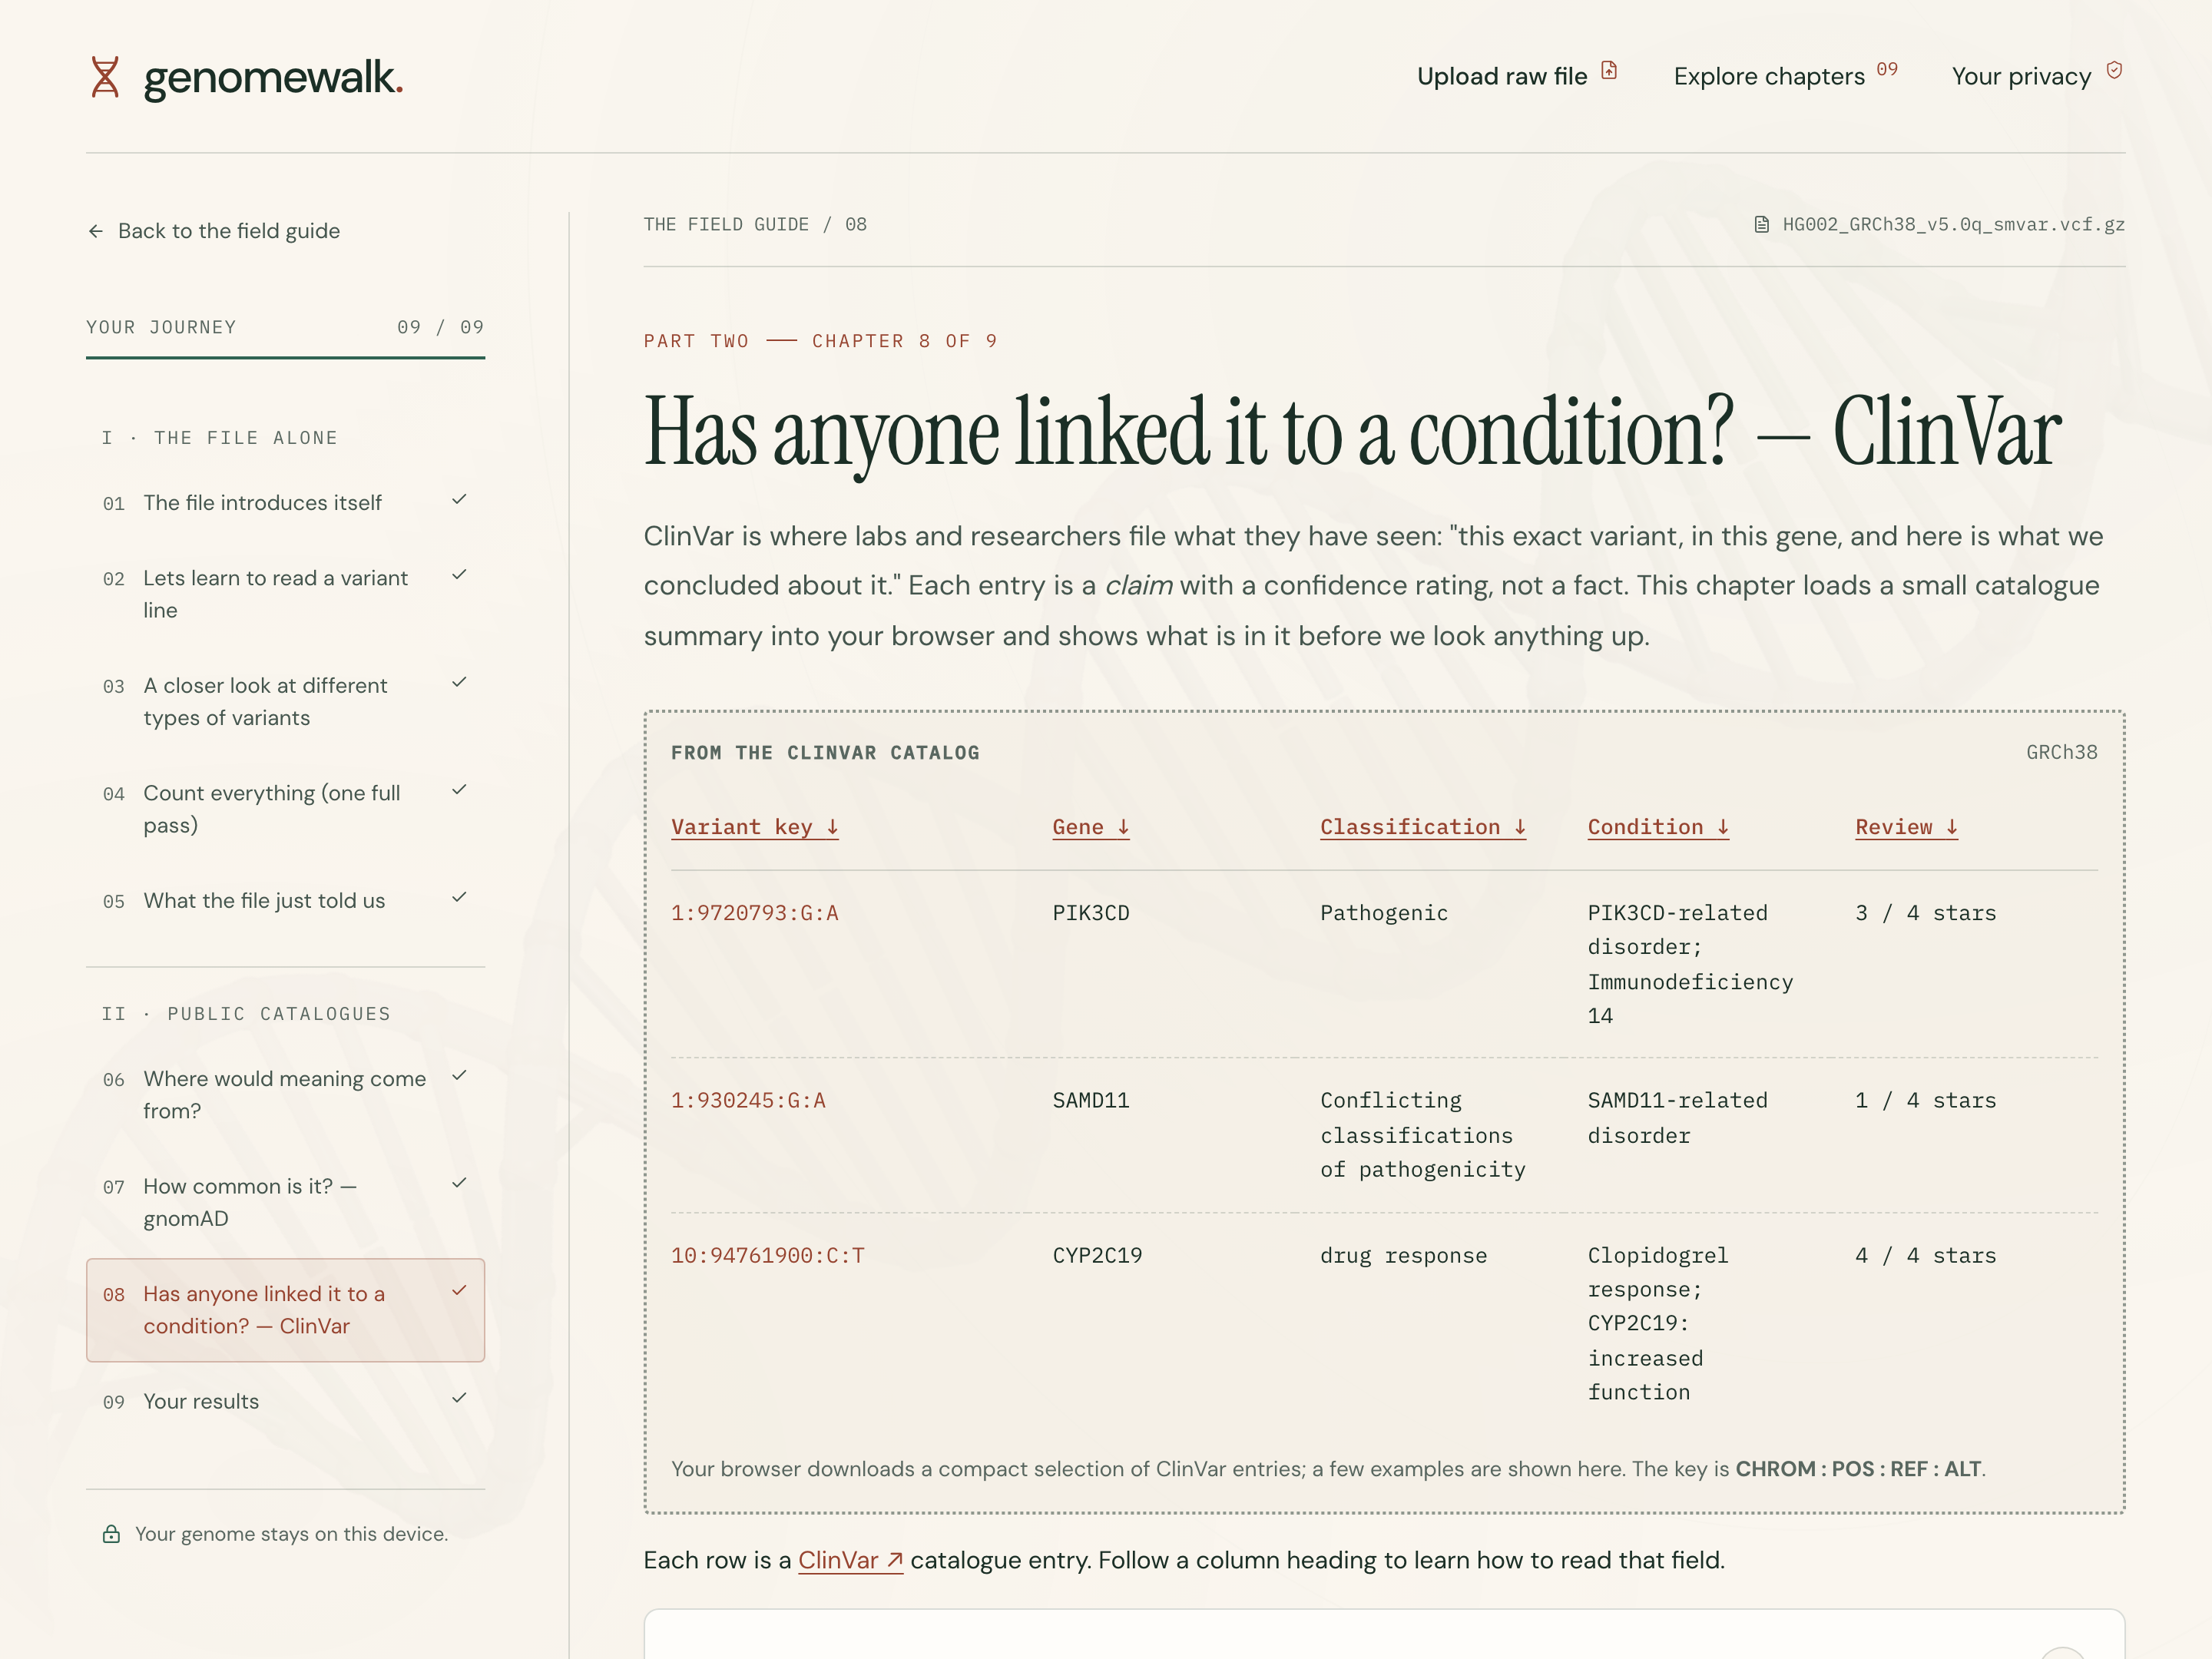
\includegraphics[width=\linewidth]{figures/chapters/chapter-08-desktop.png}
\Description{Full desktop view of Chapter 8 showing a public catalogue preview with PIK3CD, SAMD11 and CYP2C19 examples, their classifications and review stars. These are teaching entries rather than HG002 matches.}
\caption{Chapter 8 introduces ClinVar classifications and review status through a public catalogue preview.}
\label{fig:chapter-8}
\end{wrapfigure}
A public catalogue preview introduces classifications and review status before the reader reaches their matches (Fig.~\ref{fig:chapter-8}). Examples include pathogenic, conflicting and drug-response records. Linked headings lead to explanations of what the labels, stars and supporting fields describe. ClinVar stars indicate review status, including whether criteria or expert review support a classification; they do not measure disease severity~\cite{review}. These are selected public examples, not a list of variants found in HG002. The chapter prepares readers to examine the evidence attached to a result.
\finishchapterwrap
\end{minipage}\par


\par\noindent\begin{minipage}{\textwidth}
\subsection{Chapter 9: Your results}
\setlength{\intextsep}{4pt}
\setlength{\columnsep}{.04\textwidth}
\begin{wrapfigure}{r}{.50\textwidth}
\centering
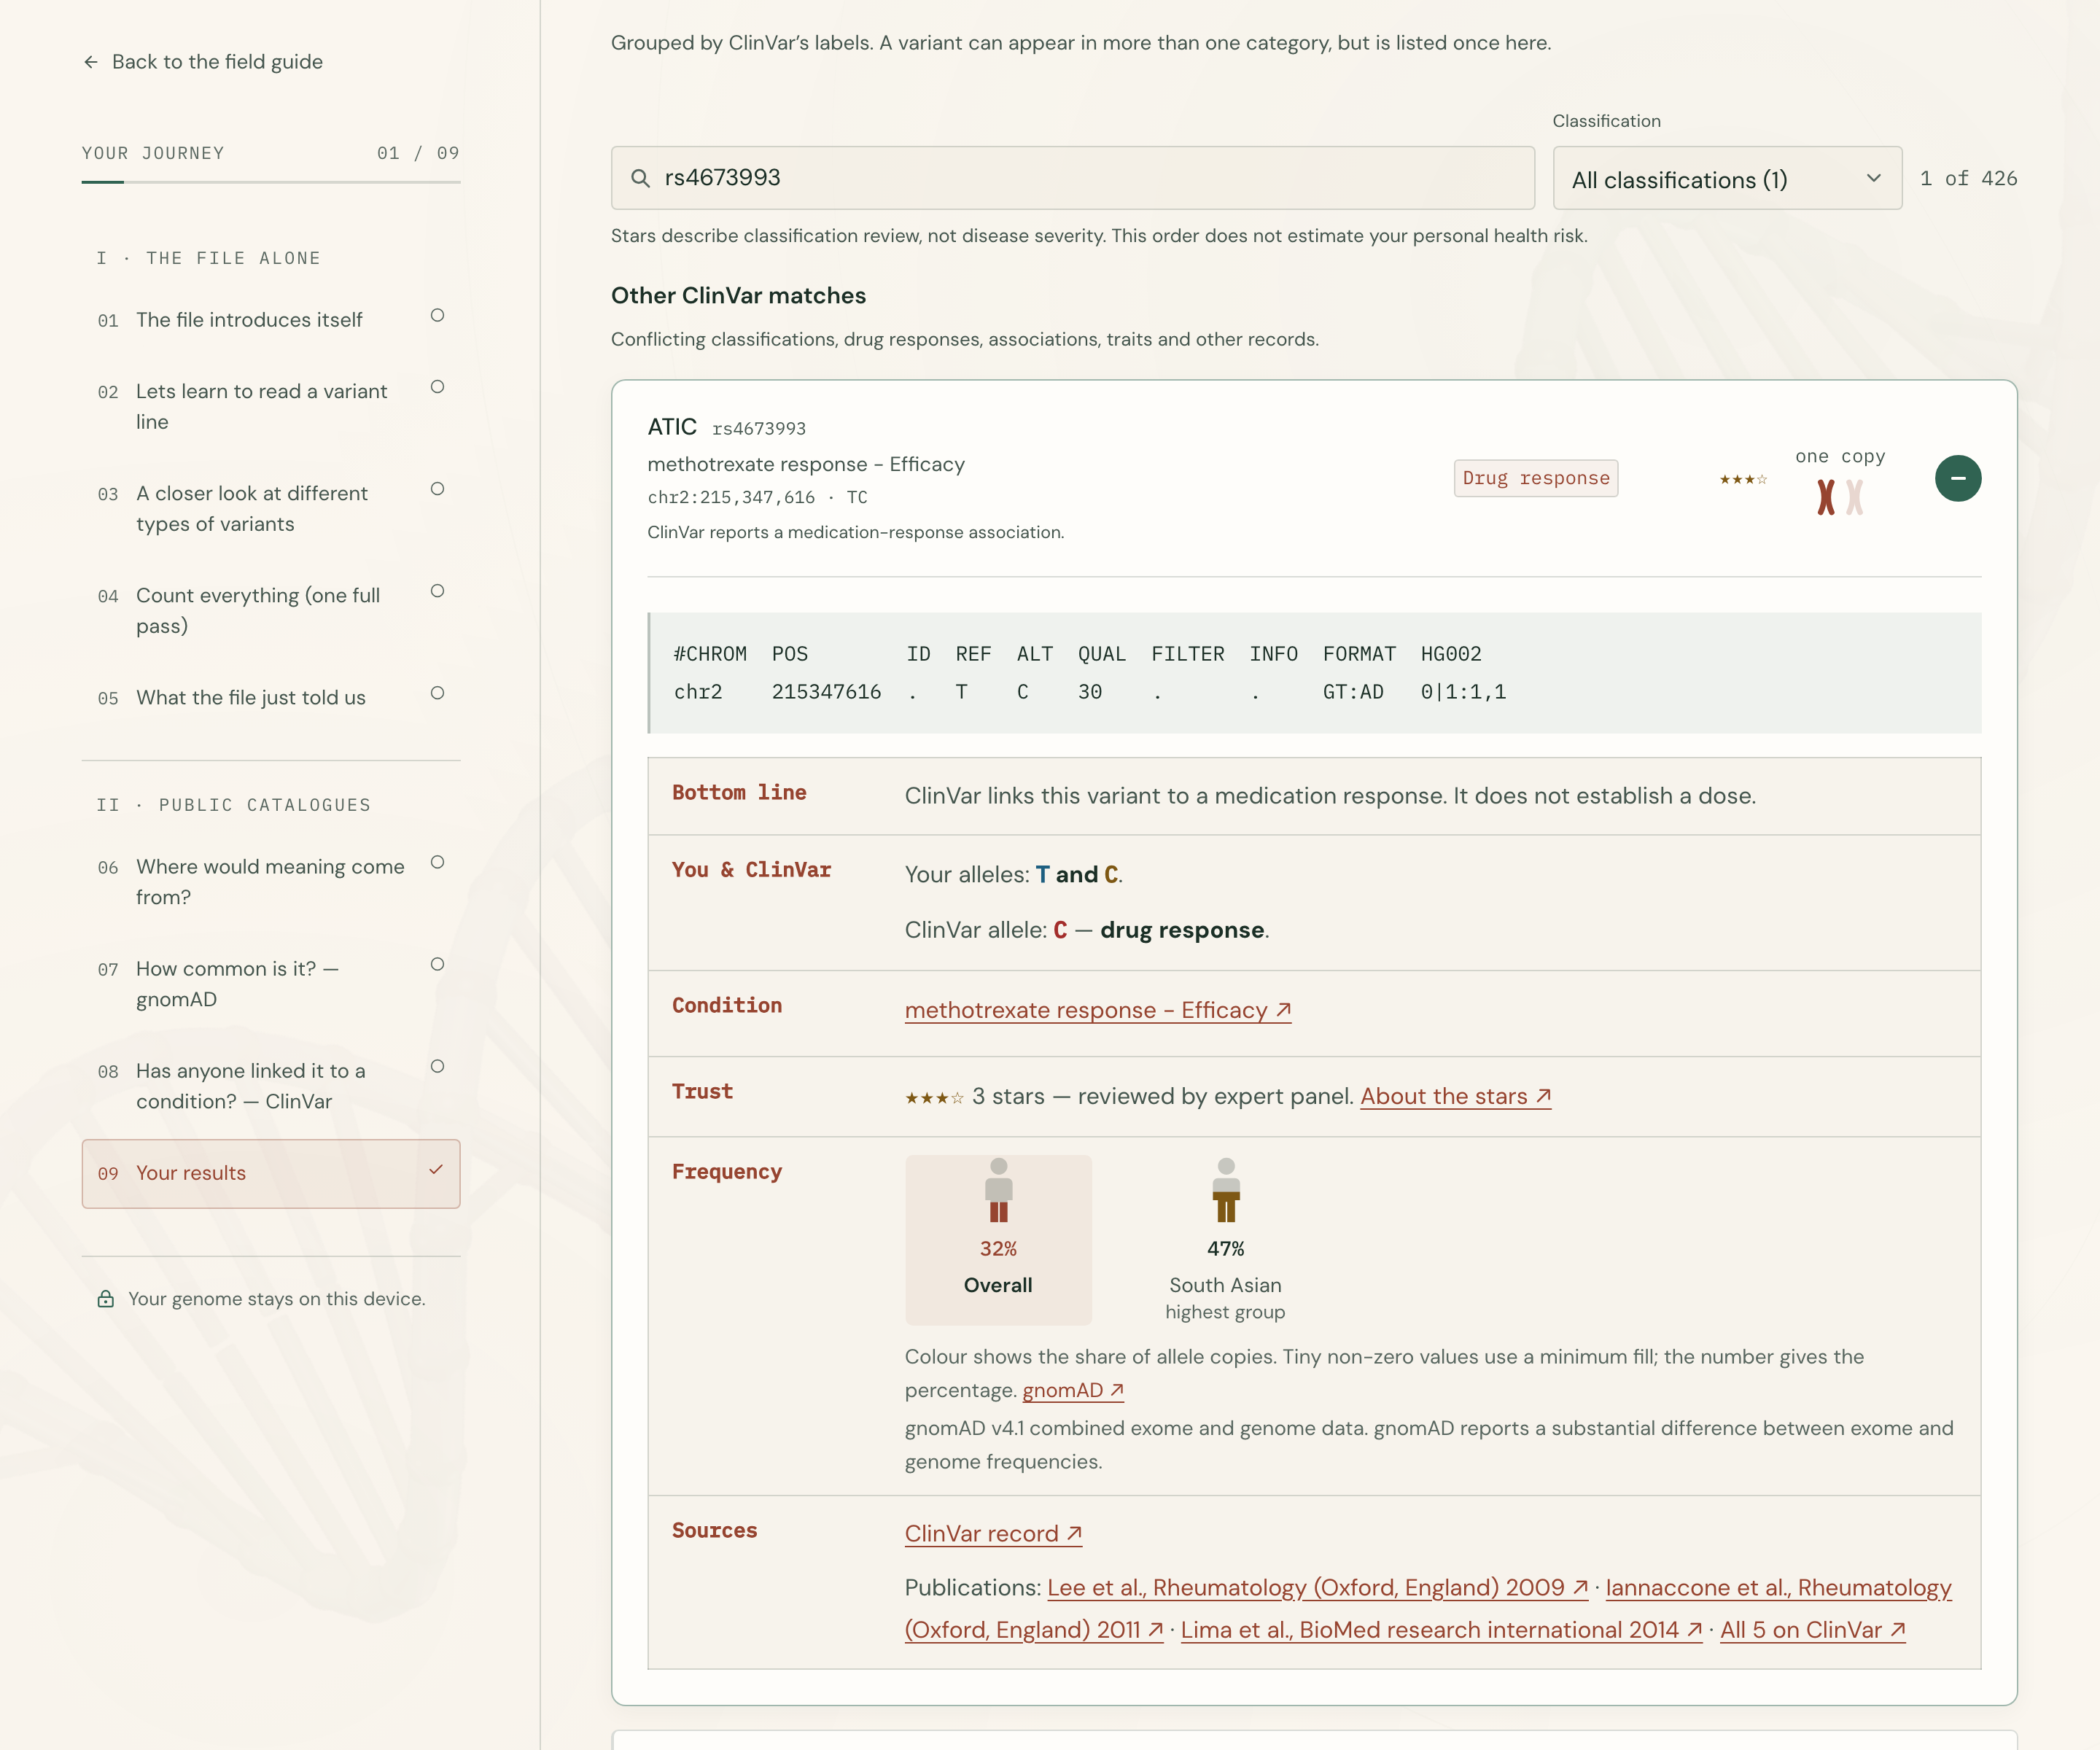
\includegraphics[width=\linewidth]{figures/chapters/chapter-09-desktop.png}
\Description{Full desktop view scrolled to an expanded HG002 result for ATIC rs4673993. Search returns one of 426 matches. The card shows the original T-to-C call with genotype 0|1, a drug-response classification, three review stars, population frequencies and source links.}
\caption{Chapter 9: an expanded HG002 match connects the local call to public evidence and its sources.}
\label{fig:chapter-9}
\end{wrapfigure}
The final chapter brings the local calls and matched public records together. Readers can search by gene, condition, identifier or position and filter by classification. Opening a result shows the original file row, the matched allele, classification, review status, population frequency and source references. Figure~\ref{fig:chapter-9} shows an actual HG002 match for \texttt{rs4673993} in \textit{ATIC}; its drug-response label is accompanied by an explanation that the record does not establish a dose.

The application orders results using classification and review information and explains that choice. This is an application-defined presentation order, not a ClinVar-recommended ranking of personal health risks. Incomplete or contradictory calls are distinguished as needing verification. Links allow readers to inspect the public sources behind a summary, completing the progression from file notation to evidence inspection.
\finishchapterwrap
\end{minipage}\par


The public Genome in a Bottle HG002 GRCh38 v5.0q sample~\cite{giab} provides a repeatable starting point for classroom activities. Learners could identify the reference build, read a variant and its genotype, and explain the evidence behind a catalogue match.

\section{Public Data Preparation and Local Processing}
\subsection{A selected and enriched public catalogue}
Automated pipelines download ClinVar records~\cite{clinvar} and prepare GRCh37 and GRCh38 catalogues. Selection retains pathogenic, likely pathogenic, combined pathogenic and likely pathogenic, and conflicting classifications, alongside supported labels such as drug response, risk factor, association and protective. Benign, likely benign or uncertain significance alone do not qualify; mixed records remain eligible when another supported classification is present. Original classification text is preserved. Selection also requires explicit reference and alternate alleles of at most 50 bases.

The pipeline adds gnomAD v4.1 combined exome/genome frequencies~\cite{gnomad} and publication references. GRCh38 joining uses exact variant identities; GRCh37 associates those frequencies through ClinVar Allele IDs. The current GRCh38 catalogue has 511,286 rows in 28.06 MB; GRCh37 has 511,282 rows in 26.88 MB (compressed decimal megabytes). Filtering reduces the download but limits coverage; it does not imply that excluded records lack value.

\begin{figure}[H]
\centering
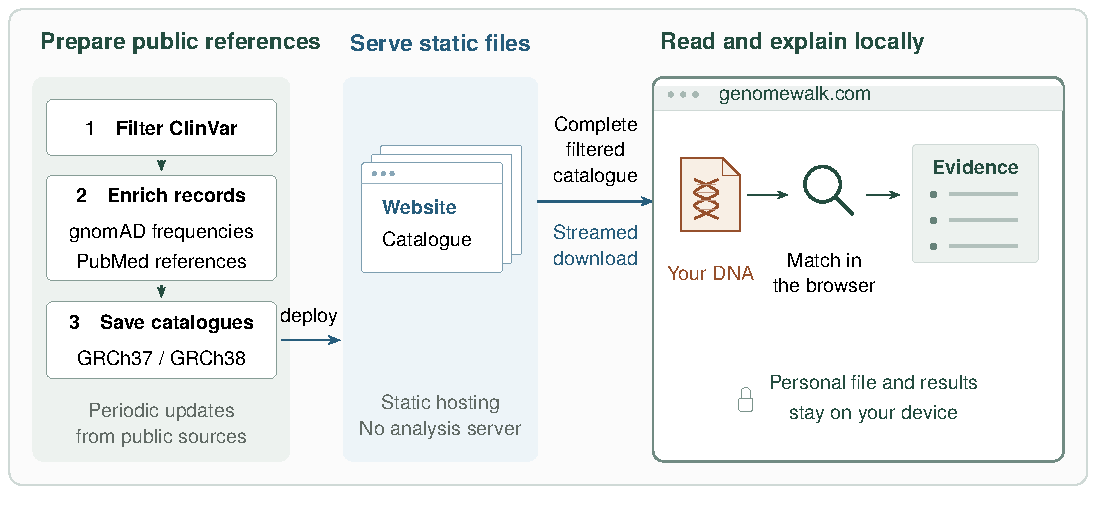
\includegraphics[width=\textwidth]{figures/figure-2-local-processing.pdf}
\Description{Three stages show public reference preparation, static hosting and local browser processing. An automated pipeline selects ClinVar records, adds gnomAD frequencies and PubMed citation labels, and saves filtered GRCh37 and GRCh38 catalogues. The static host streams the complete relevant catalogue to the browser, where a locally read personal genome is matched to public evidence. Personal files and results remain on the device.}
\caption{Public references are prepared before deployment. The browser receives the complete filtered catalogue and combines it with the locally read genome file. Personal files and results are not uploaded for processing.}
\label{fig:processing}
\end{figure}

\subsection{Local reading and matching}
The browser streams the complete relevant catalogue in blocked gzip (BGZF) format (Fig.~\ref{fig:processing}), decompresses it progressively and releases processed data. For a VCF and catalogue in compatible chromosome/position order, a streaming merge join compares exact alleles at shared positions and retains matches. Catalogue integrity is checked before successful completion. Unsorted VCFs and consumer exports use a compatibility path that retains compact public identities before a second complete catalogue pass retains matching rows. Input buffers and accumulated results can still grow; streaming is not a fixed memory guarantee.

Supported inputs include BGZF-compressed Variant Call Format (VCF) and genomic VCF (gVCF) files, and original 23andMe or AncestryDNA raw exports. Matching is build-specific and uses the first VCF sample with the application's genotype and filter rules. Chromosome aliases are handled, but indels are not normalized and coordinates are not lifted between builds. These constraints affect which records appear in the results.

For HG002, the streaming matcher and a simpler reference calculation returned the same 426 records, with agreement on every field and result order. Both used the same catalogue and shared parsing and annotation helpers; the reproducible check is available in the project repository~\cite{genomewalk}.

\subsection{Privacy boundaries}
Personal files, filenames, genotypes and derived results remain on the device and are excluded from application analytics. Limited usage and diagnostic events may contain processing stages, fixed error codes, recognized formats, approximate size bands and coarse browser information. Session recording and automatic interaction capture are disabled. Source code and privacy documentation are available for inspection~\cite{genomewalk}.

Hosting and analytics endpoints see connection metadata. Hosts see catalogue and reference-file requests; external evidence links reveal the requested record to the destination service. Application delivery, the browser and the device remain part of the trust boundary. No independent security audit is claimed.

\section{Conclusion and Further Work}
Genomewalk brings genomic file reading and public evidence into a guided, browser-based learning experience. Its nine chapters provide a starting point for introductory teaching and independent exploration, with a public HG002 sample for shared activities and local processing for readers who choose to explore their own genome.

Further development should be guided by learners and instructors. Additional chapters and practical exercises may be needed to address gaps in the current walkthrough or support different levels of prior knowledge. Instructor feedback is needed to assess the explanations, identify missing topics and shape activities that fit existing courses.

No user study has yet been conducted. Studies using the public sample should examine how people respond to the interface, where they become confused and whether they learn to read genomic records and assess the evidence behind a match. Observing tasks and comparing explanations before and after the walkthrough would help assess changes in understanding. Asking learners to apply what they learned to an unfamiliar record would also help distinguish understanding from simply following the steps. These findings should guide revisions to the content and interface.

We are seeking collaborations with genomics laboratories, schools and universities to review the material, develop classroom activities and evaluate the learning experience. Interested educators and researchers can contact \mbox{\href{mailto:genomewalk123@gmail.com}{genomewalk123@gmail.com}}.

\begin{thebibliography}{8}
\bibitem{gnomad}
Chao, K., Wilson, M., Goodrich, J., gnomAD Production Team: gnomAD v4.1 (2024). \url{https://gnomad.broadinstitute.org/news/2024-04-gnomad-v4-1}
\bibitem{genomewalk}
Genomewalk: Source code, documentation and correctness benchmark. \url{https://github.com/genomewalk/genomewalk}. Application: \url{https://genomewalk.com} (accessed November 2026)
\bibitem{interpretome}
Karczewski, K.J., et al.: Interpretome: a freely available, modular, and secure personal genome interpretation engine. In: Pacific Symposium on Biocomputing, vol.~17, pp.~339--350 (2012). \url{https://psb.stanford.edu/psb-online/proceedings/psb12/karczewski.pdf}
\bibitem{clinvar}
Landrum, M.J., et al.: ClinVar: updates to support classifications of both germline and somatic variants. Nucleic Acids Research \textbf{53}(D1), D1313--D1321 (2025). \doi{10.1093/nar/gkae1090}
\bibitem{myseq}
Linderman, M.D., McElroy, L., Chang, L.: MySeq: privacy-protecting browser-based personal genome analysis for genomics education and exploration. BMC Medical Genomics \textbf{12}, 172 (2019). \doi{10.1186/s12920-019-0615-3}
\bibitem{cyanohabit}
Matthews, E.A., Matthews, R.A., Sheets, Z., Gilbert, J.E.: CyanoHABIT: a novel game to identify harmful freshwater algae. In: HCI International 2018 -- Posters' Extended Abstracts. CCIS, vol.~852, pp.~78--84. Springer (2018). \doi{10.1007/978-3-319-92285-0_12}
\bibitem{review}
National Center for Biotechnology Information: ClinVar review status. \url{https://www.ncbi.nlm.nih.gov/clinvar/docs/review_status/} (accessed November 2026)
\bibitem{giab}
NIST / Genome in a Bottle Consortium: HG002 GRCh38 v5.0q small-variant benchmark release. \url{https://ftp-trace.ncbi.nlm.nih.gov/ReferenceSamples/giab/release/AshkenazimTrio/HG002_NA24385_son/v5.0q/} (accessed November 2026)
\end{thebibliography}
\end{document}
